\documentclass[12pt]{article}

%paquetes del idioma y codificacion
\usepackage[spanish]{babel}
\usepackage[utf8]{inputenc}
\usepackage[T1]{fontenc}
\usepackage{bookman}

%el indice
\usepackage{makeidx}

%paquetes matematicos
\usepackage{amsmath, amsfonts, amssymb}

%dimensiones
\usepackage[left=2.5cm, right=2.5cm, top=3cm]{geometry}

%para escribir codigo
\usepackage{listings}

% para contraer referencias
\usepackage{url}
\usepackage{cite}

%para las imagenes y mas...
\usepackage{graphicx}
\usepackage{subfig}
\graphicspath{ {imagenes/} }
\usepackage{float}

\usepackage[nottoc,numbib]{tocbibind}


\title{Reporte de prácticas del primer periodo}
\author{Ian Mendoza Jaimes}
\date{}



\begin{document}


\maketitle

\begin{center}
\large
2CM4

Teoría Computacional

Profesor Genaro Juaréz Martínez
\end{center}

\newpage

\tableofcontents

\newpage


\section{Universo de palabras}
Los alfabetos se definen como un conjunto finito, no vacío de símbolos. Comúnmente se denotan con la letra griega $\sum$. Al definir un alfabeto, podemos tener acceso a seleccionar un conjunto finito de estos símbolos, a esto se le llama cadena o string. \cite{automatas}

\subsection{Descripción del problema}
Se necesita realizar un programa, que dado un alfabeto binario $\sum = \lbrace 0, 1 \rbrace $ en este caso, sea  capaz  de calcular e imprimir en un archivo de texto todas las palabras que puedan ser formadas por un alfabeto binario, es decir, \[{\sum}^{*} = {\sum}^{0}\cup{\sum}^{1}\cup{\sum}^{2}\cup\cdots\] Sin embargo, tiene limitaciones, pues es imposible calcular algo infinito, el programa deberá imprimir todas las combinaciones de las palabras con la longitud: $0 \leq n \leq 1000$.

\subsection{Código fuente}
El programa para este problema fue escrito en el lenguaje C. Esto debido a su alta velocidad de procesamiento, la cual es bastante necesaria si la longitud de las palabras es grande. El código utilizado para la resolución del problema se muestra a continuación:\\

Archivo: main.c
\lstset{language=C, breaklines=true, basicstyle=\footnotesize}
\begin{lstlisting}[frame=single]
#include "alfabeto.h"

int main(int argc, char const *argv[]) {
    char seleccion = '1';
    int continuar = 1;
    int continuar_modalidad = 1;
    int n = 0;
    char seleccion_tiro = ' ';

    srand(time(NULL));

    while(continuar == 1){
        printf("%s\n", "Seleccione la modalidad: \n1.- Automatico \n2.- Manual \n3.- Salir");
        scanf(" %c", &seleccion);

        if(seleccion == '1' || seleccion == '2'){
            continuar_modalidad = 1;
            while (continuar_modalidad == 1) {
                if(seleccion == '1'){
                    n = 1  + (rand()%5);
                }
                else{
                    printf("%s ", "Ingrese un n: ");
                    scanf("%d", &n);
                }

                iniciar_programa(n);

                if(seleccion == '2'){
                    printf("%s\n", "Desea ingresar otra n?: s/n");
                    scanf(" %c", &seleccion_tiro);
                    if(seleccion_tiro == 's' || seleccion_tiro == 'S'){
                        continuar_modalidad = 1;
                    }
                    else{
                        continuar_modalidad = 0;
                    }
                }
                else{
                    continuar_modalidad = rand()%2;
                    printf("%d\n", continuar_modalidad);
                }
            }
        }
        else{
            return 1;
        }
    }


    return 0;
}
}
\end{lstlisting}

\vspace{1em}
Archivo: alfabeto.c
\lstset{language=C, breaklines=true, basicstyle=\footnotesize}
\begin{lstlisting}[frame=single]
#include "alfabeto.h"

int iniciar_programa(int n){
  int tamanio_alfabeto = 2;
  char * alfabeto = NULL;
  alfabeto = (char *)malloc(tamanio_alfabeto * sizeof(char));
  iniciar_alfabeto(&alfabeto, tamanio_alfabeto);

  obtener_cadenas(alfabeto, tamanio_alfabeto, n);

  return 1;
}


int obtener_cadenas(char *alfabeto, int tamanio, int n){
    int i;
    int j;
    int * cadena_temporal = NULL;
    int salir = 0;

    FILE *archivo = NULL;

    archivo = fopen("cadenas.txt", "w");
    if (archivo == NULL) {
		printf("%s\n", "Error al abrir el archivo");
		exit(0);
	}

    fputs(" = { ", archivo);

    for(i = 1; i <= n; i++){
        cadena_temporal = (int*)calloc(i, sizeof(int));
        while(salir == 0){
            escribir_palabra(archivo, cadena_temporal, alfabeto, i);
            for(j = i -1; j > -1; j--){
                *(cadena_temporal + j) = *(cadena_temporal + j) + 1;
                if( *(cadena_temporal + j) > (tamanio -1)){
                    *(cadena_temporal + j) = 0;
                }
                else{break;}
            }
            if(j == -1){
                free(cadena_temporal);
                break;
            }
        }
        printf("Va en n = %d\n", i);
    }
    fputs(" }", archivo);
    fclose(archivo);

    return 1;
}

int escribir_palabra(FILE *archivo, int * cadena_temporal, char * alfabeto, int tamanio){
    int i;
    fputs(", ", archivo);
    for(i = 0; i < tamanio; i++){
        fputc(*(alfabeto + *(cadena_temporal + i)) , archivo);
    }
    return 1;
}

int iniciar_alfabeto(char **alfabeto, int tamanio){
    int i;
    for(i = 0; i < tamanio; i++){
        *(*alfabeto + i) = i + '0';
    }
    return  1;
}
\end{lstlisting}

\vspace{1em}
Archivo: alfabeto.h
\lstset{language=C, breaklines=true, basicstyle=\footnotesize}
\begin{lstlisting}[frame=single]
#ifndef __ALFABETO_H__
#define __ALFABETO_H__

#include <stdio.h>
#include <string.h>
#include <stdlib.h>
#include <time.h>


int iniciar_programa();
int iniciar_alfabeto(char **, int);
int escribir_palabra(FILE *, int *,char*, int);
int obtener_cadenas(char *, int, int);

#endif
\end{lstlisting}

\newpage
\subsection{Pruebas}
En cuanto a las pruebas, a continuación se mostraran una serie de imágenes capturadas al momento de ejecutar el programa. Los resultados arrojados por el programa anterior son:\\

Para la selección en modo automático:

\begin{figure}[H]
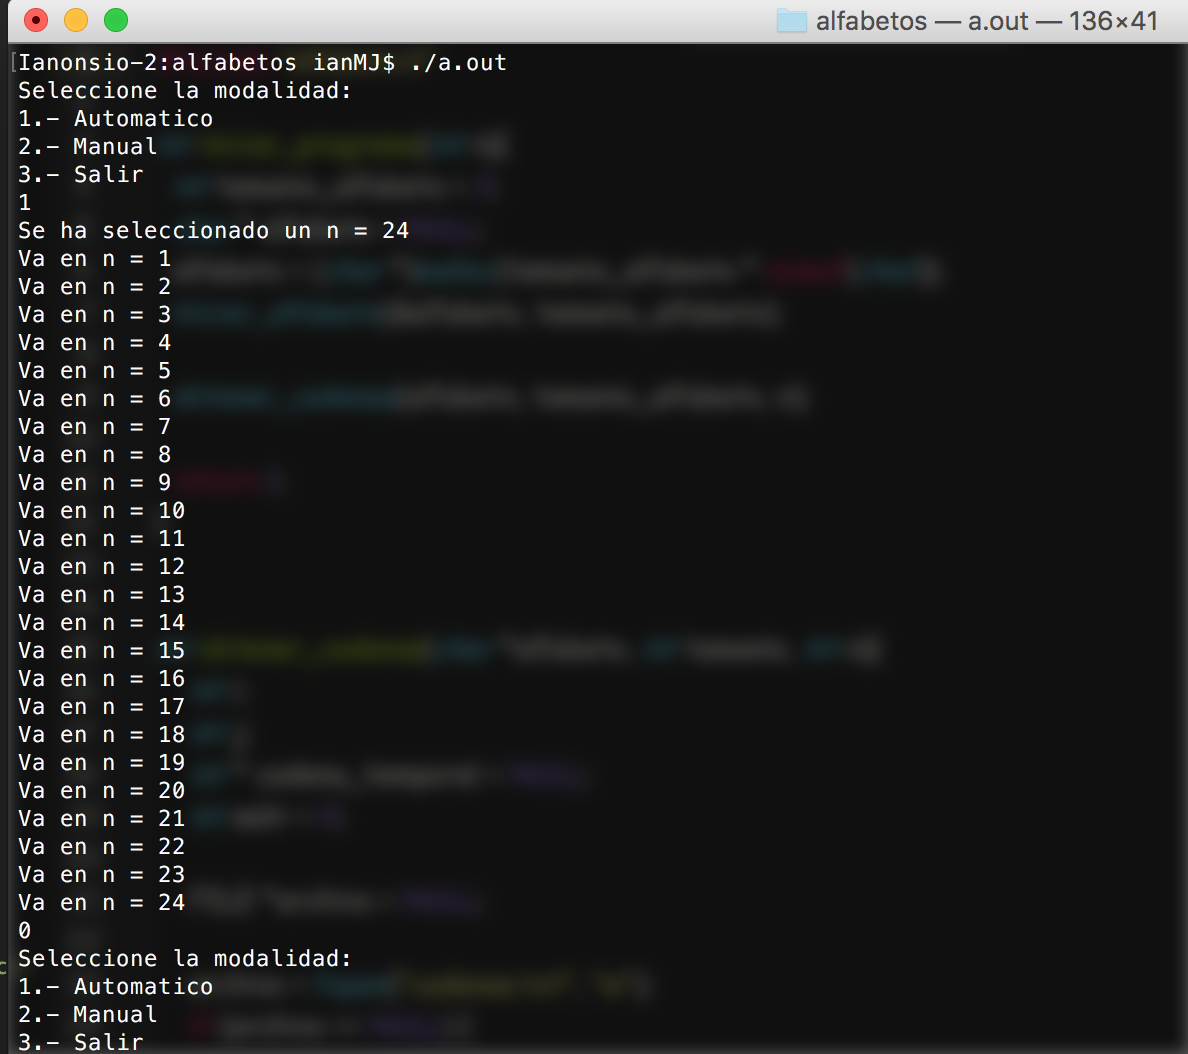
\includegraphics[width=\textwidth, height=7cm]{alfabetos_automatico}
\label{fig:auto_alfabeto}
\caption{Selección de un n = 24 de forma automática.}
\end{figure}

\vspace{1em}

\begin{figure}[H]
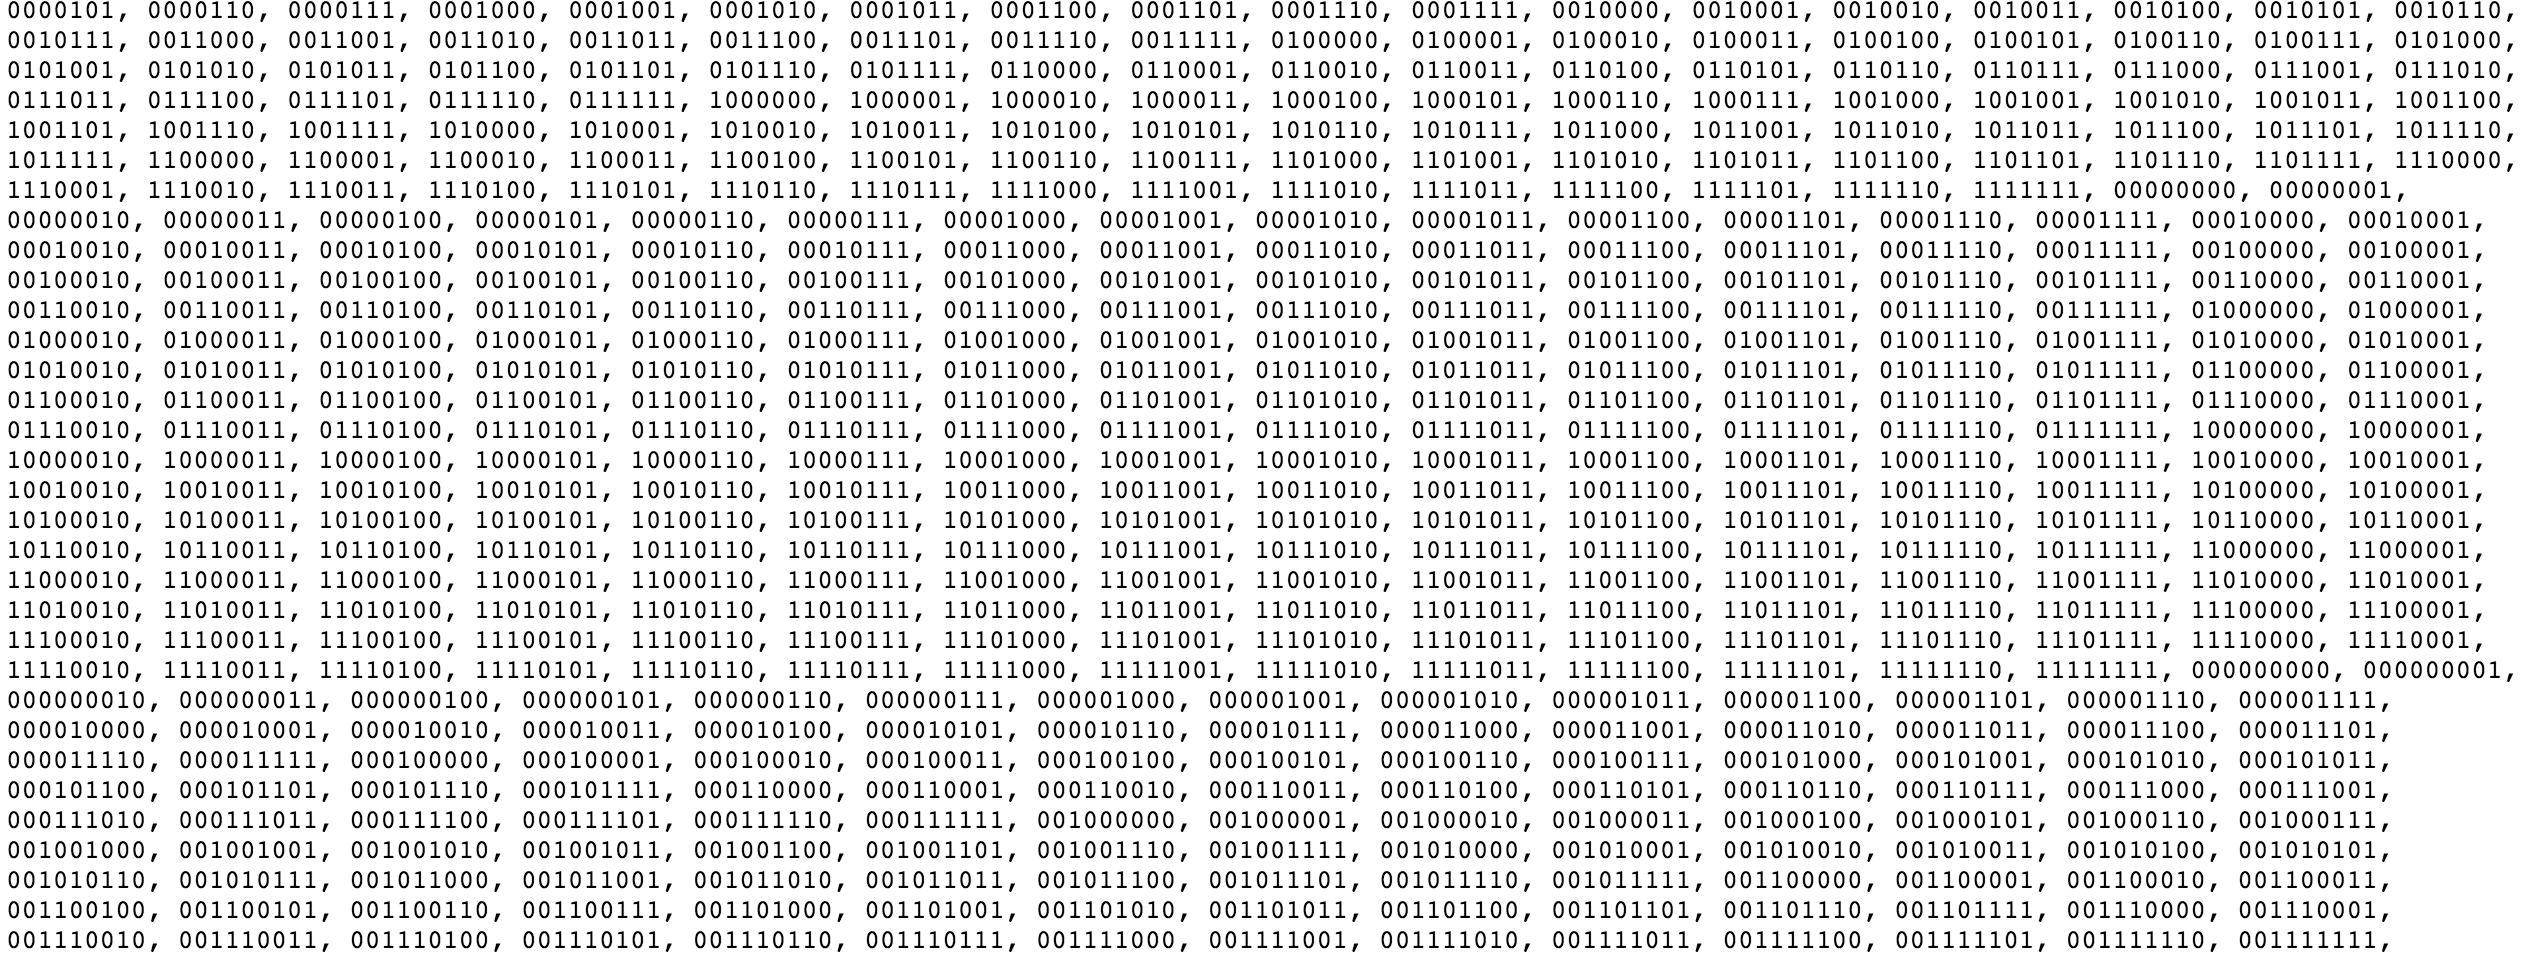
\includegraphics[width=\textwidth, height=6cm]{alfabeto_muestra}
\label{fig:auto_alfabeto_texto}
\caption{Texto producido por un n = 24.}
\end{figure}

\vspace{1em}

Para la selección en modo manual:

\begin{figure}[H]
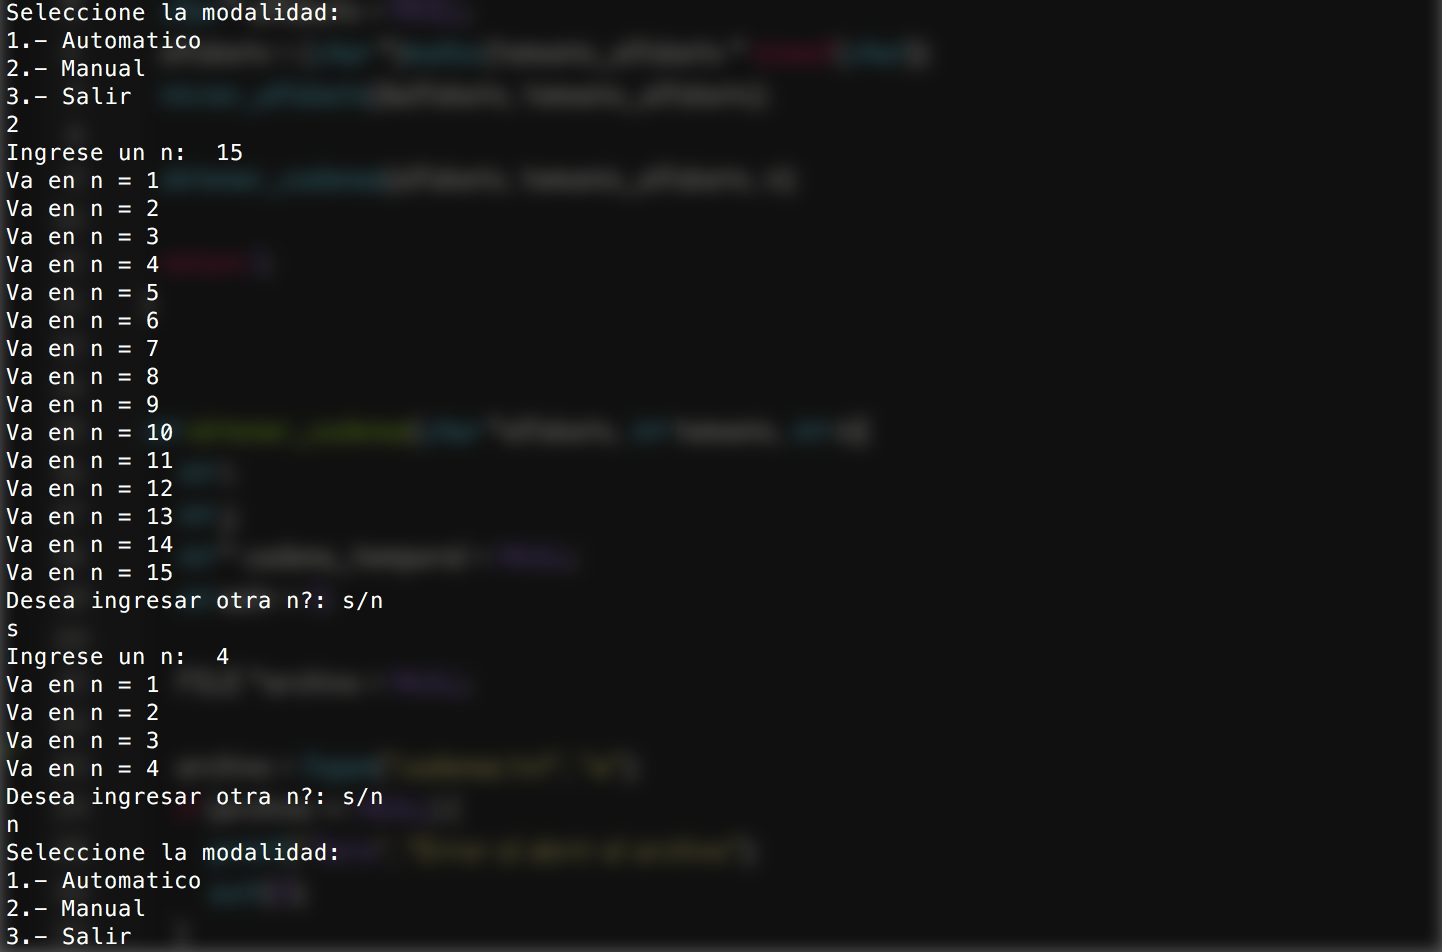
\includegraphics[width=\textwidth, height=7cm]{alfabetos_manual}
\label{fig:manual_alfabeto}
\caption{El resultado de escoger manualmente a n.}
\end{figure}

\begin{figure}[H]
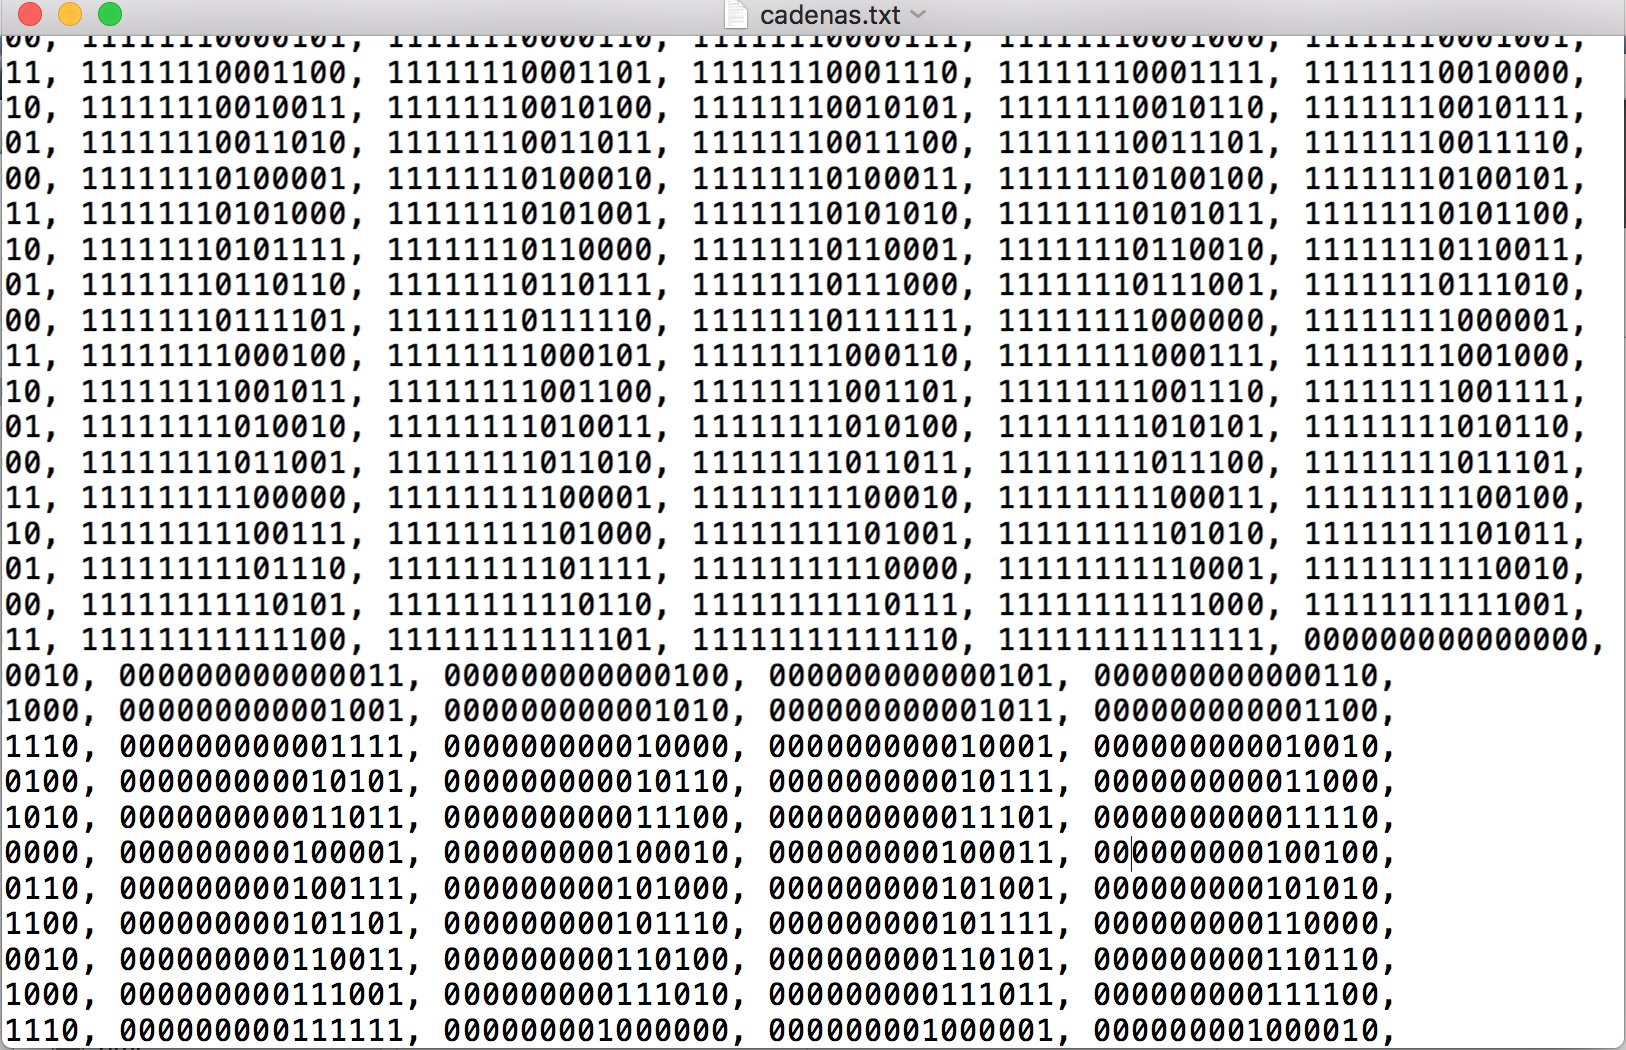
\includegraphics[width=\textwidth, height=10cm]{alfabeto_muestra_manual}
\caption{Texto producido por n = 15.}
\label{fig:manual_alfabeto_texto}
\end{figure}

%===============================================================================================
%===============================================================================================
%===============================================================================================
%===============================================================================================
%===============================================================================================
%===============================================================================================
%===============================================================================================
%===============================================================================================
\newpage
\section{Números primos}
Un número primo es aquel que solo puede ser divido entre si mismo o la unidad. A lo largo de la historia mucha gente los a estudiado y han propuesto numerosas maneras de encontrarlos. Algunos ejemplos de ello son la criba de Eratóstenes o la criba de Euler. En esta sección presentaremos un programa capaz de calcular todos los números primos en un intervalo dado.

\subsection{Descripción del problema}
Realizar un programa capaz de encontrar todos los números primos dentro de un intervalo dado por: $0 \leq n \leq 1000$. Además, deberá convertir dichos números de su representación decimal a su representación binaria y guardarlos en un archivo de texto. Después, se debe proceder a graficar la cantidad de ceros y unos que aparecen dependiendo de n.

\subsection{Código}
El programa, en este caso, fue escrito en Python. Fue seleccionado este lenguaje por la facilidad que presenta al manejar estructuras de datos como listas, pilas, etc. A continuación se presenta el código utilizado:\\


Archivo: main\_primos.py
\lstset{language=Python, breaklines=true, basicstyle=\footnotesize}
\begin{lstlisting}[frame = single]
from metodos import *
from random import random

def main():
    archivo = open("primos.txt", "w")
    archivo.write("")
    archivo.close()
    seguir = True
    while seguir:
        print("\n\nSelecciona el modo en que se ejecutara el programa: \n 1.- Automatico \n 2.- Manual \n 3.- Salir")
        try:
            seleccion = int(input())
            if seleccion > 0 and seleccion <= 2:
                iniciar_programa(seleccion)
            elif seleccion == 3:
                return 1;
            else:
                raise Exception()
        except Exception as e:
            print("Por favor ingrese un dato valido.")


def iniciar_programa(seleccion=1):
    numeros_primos = []
    numeros_primos_binarios = []
    numero_ceros_unos = []
    n = 0
    continuar = True
    archivo = None

    while continuar:
        if seleccion == 2:
            n = ingresar_datos("\nIngrese un numero limite ( 0 < n <= 1000): ")
        else:
            n = int(random() * 1000)
            print("\nFue seleccionado un n = ", n)

        archivo = open("primos.txt", "a")

        numeros_primos = encontrar_primos(numeros_primos, n)
        numeros_primos_binarios = convertir_primos_a_binarios(numeros_primos, archivo, n)
        numero_ceros_unos = contar_ceros_unos(numeros_primos_binarios)

        archivo.close()

        imprimir_ceros_unos(numero_ceros_unos, numeros_primos, n)

        if seleccion == 1:
            continuar = int(random() * 100) % 2
        else:
            eleccion = ingresar_datos("\nDesea ingresar otra n?  \n1.- Si \n2.- No \n")
            if eleccion != 1:
                continuar = False


def ingresar_datos(texto):
    while True:
        try:
            dato_n = int(input(texto))
            if dato_n > 0 and dato_n <= 1000:
                return dato_n
            else:
                raise Exception()
        except Exception as e:
            print("Por favor ingrese un dato valido", e)


def imprimir_ceros_unos(numero_ceros_unos, numeros_primos, n):
    if n == 1:
        return -1

    contador = 0
    i = 0
    print('[ ', end=' ')
    try:
        while numeros_primos[i] <= n:
            print (str(numeros_primos[i])+',', end=' ')
            i += 1
    except Exception as e:
        pass
    print(']')

    print("[ numero primo, numero de unos, numero de ceros ]")
    while contador < len(numero_ceros_unos):
        print("[",numeros_primos[contador], ",",numero_ceros_unos[contador][1], ",",numero_ceros_unos[contador][0],"]", end=", ")
        contador += 1


main()

\end{lstlisting}

\vspace{1em}

Archivo: metodos\_primos.py
\lstset{language=Python, breaklines=true, basicstyle=\footnotesize}
\begin{lstlisting}[frame=single]
def encontrar_primos(numeros_primos, n):
    if n == 1:
        return numeros_primos

    if len(numeros_primos) == 0:
        numeros_primos.append(2)

#    for x in range(2,n+1):
    x = 2
    if n >= 2:
        for y in numeros_primos:
            if x%y == 0:
                es_primo = False
                break

    x = 3
    while x <= n:
        es_primo = True

        for y in numeros_primos:
            if x%y == 0:
                es_primo = False
                break

        if es_primo:
            numeros_primos.append(x)

        x += 2

    return numeros_primos


def convertir_primos_a_binarios(numeros_primos, archivo, n):
    numeros_primos_binarios = []
    for x in numeros_primos:
        if x <= n:
            numeros_primos_binarios.append(bin(x)[2:])
            archivo.write(", " + bin(x)[2:])
        else:
            break

    return numeros_primos_binarios


def contar_ceros_unos(numeros_primos_binarios):
    numero_ceros_unos = []
    contador_ceros = 0
    contador_unos = 0
    for x in numeros_primos_binarios:
        contador_unos = 0
        contador_ceros = 0
        for y in x:
            if y == '0':
                contador_ceros += 1
            else:
                contador_unos += 1

        numero_ceros_unos.append([contador_ceros, contador_unos])

    return numero_ceros_unos
\end{lstlisting}

\newpage

\subsection{Pruebas}
A continuación, se mostraran las imágenes de los resultados de ejecutar el programa en consola.\\

Para la selección de modo automático:
\begin{figure}[H]
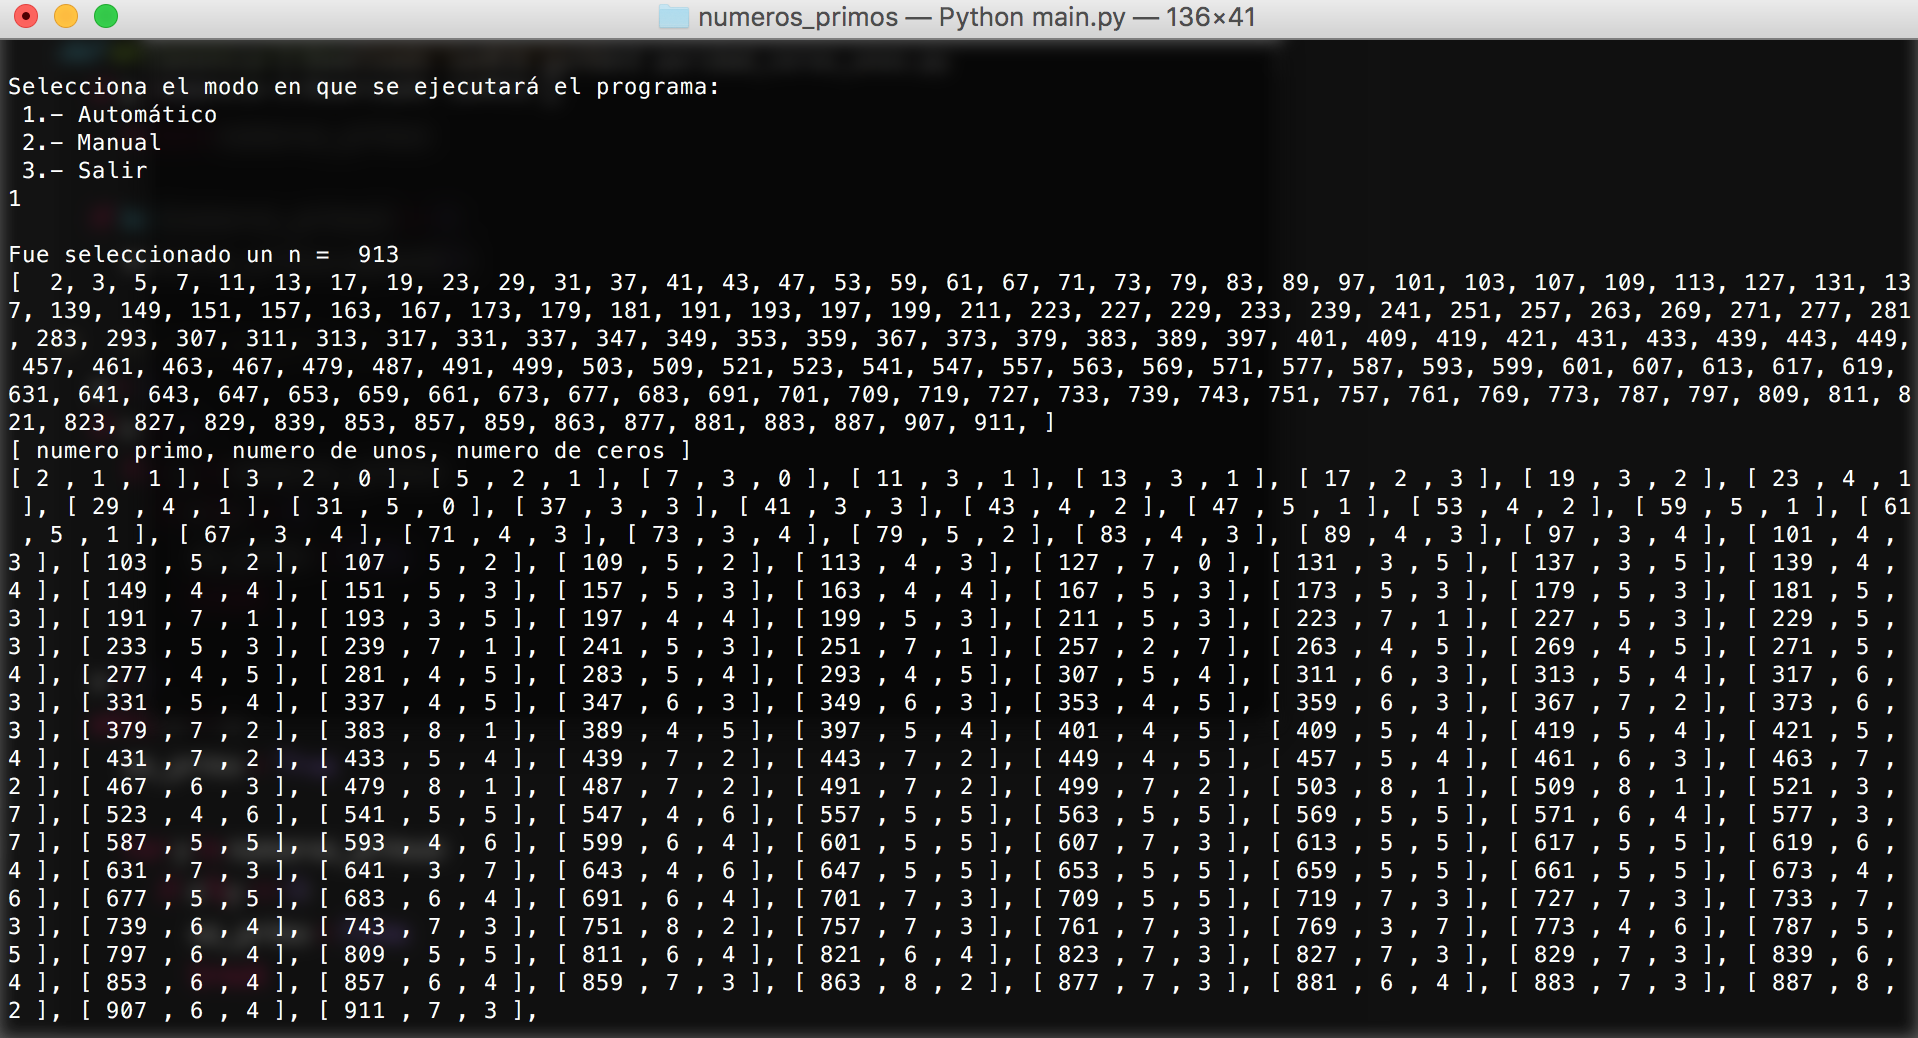
\includegraphics[width=\textwidth, height=7cm]{primos_automatico}
\caption{El resultado de seleccionar la modalidad automática.}
\label{fig:primos_automatico}
\end{figure}

\begin{figure}[H]
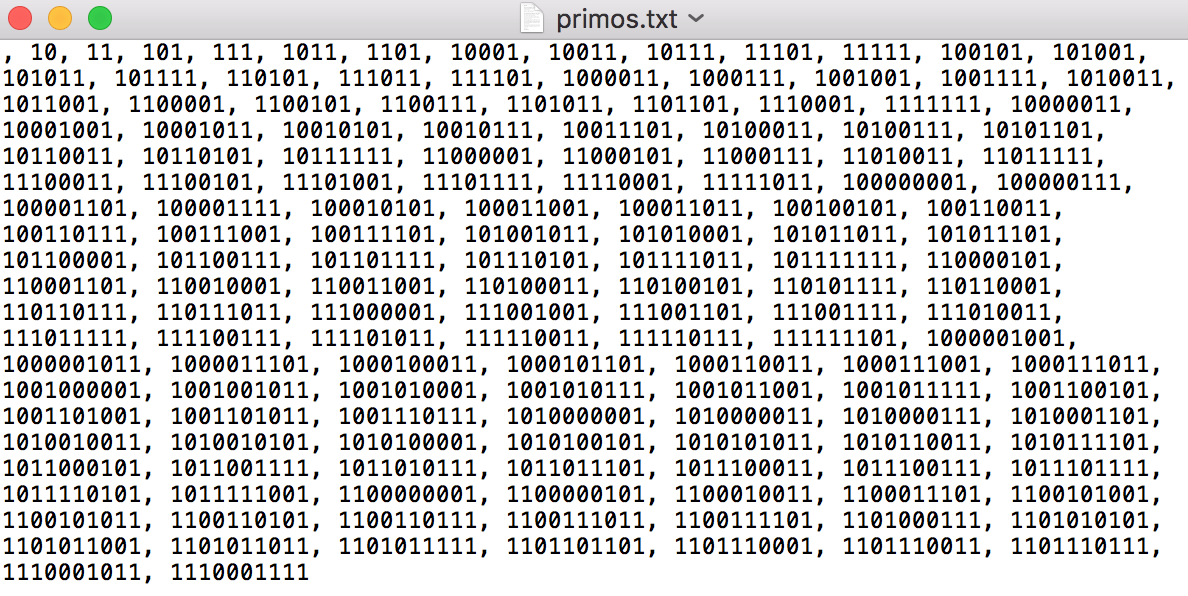
\includegraphics[width=\textwidth, height=7cm]{primos_automatico_texto}
\caption{El resultado en texto de seleccionar la modalidad automática.}
\label{fig:primos_automatico}
\end{figure}

\vspace{3em}

Para la selección manual:
\begin{figure}[H]
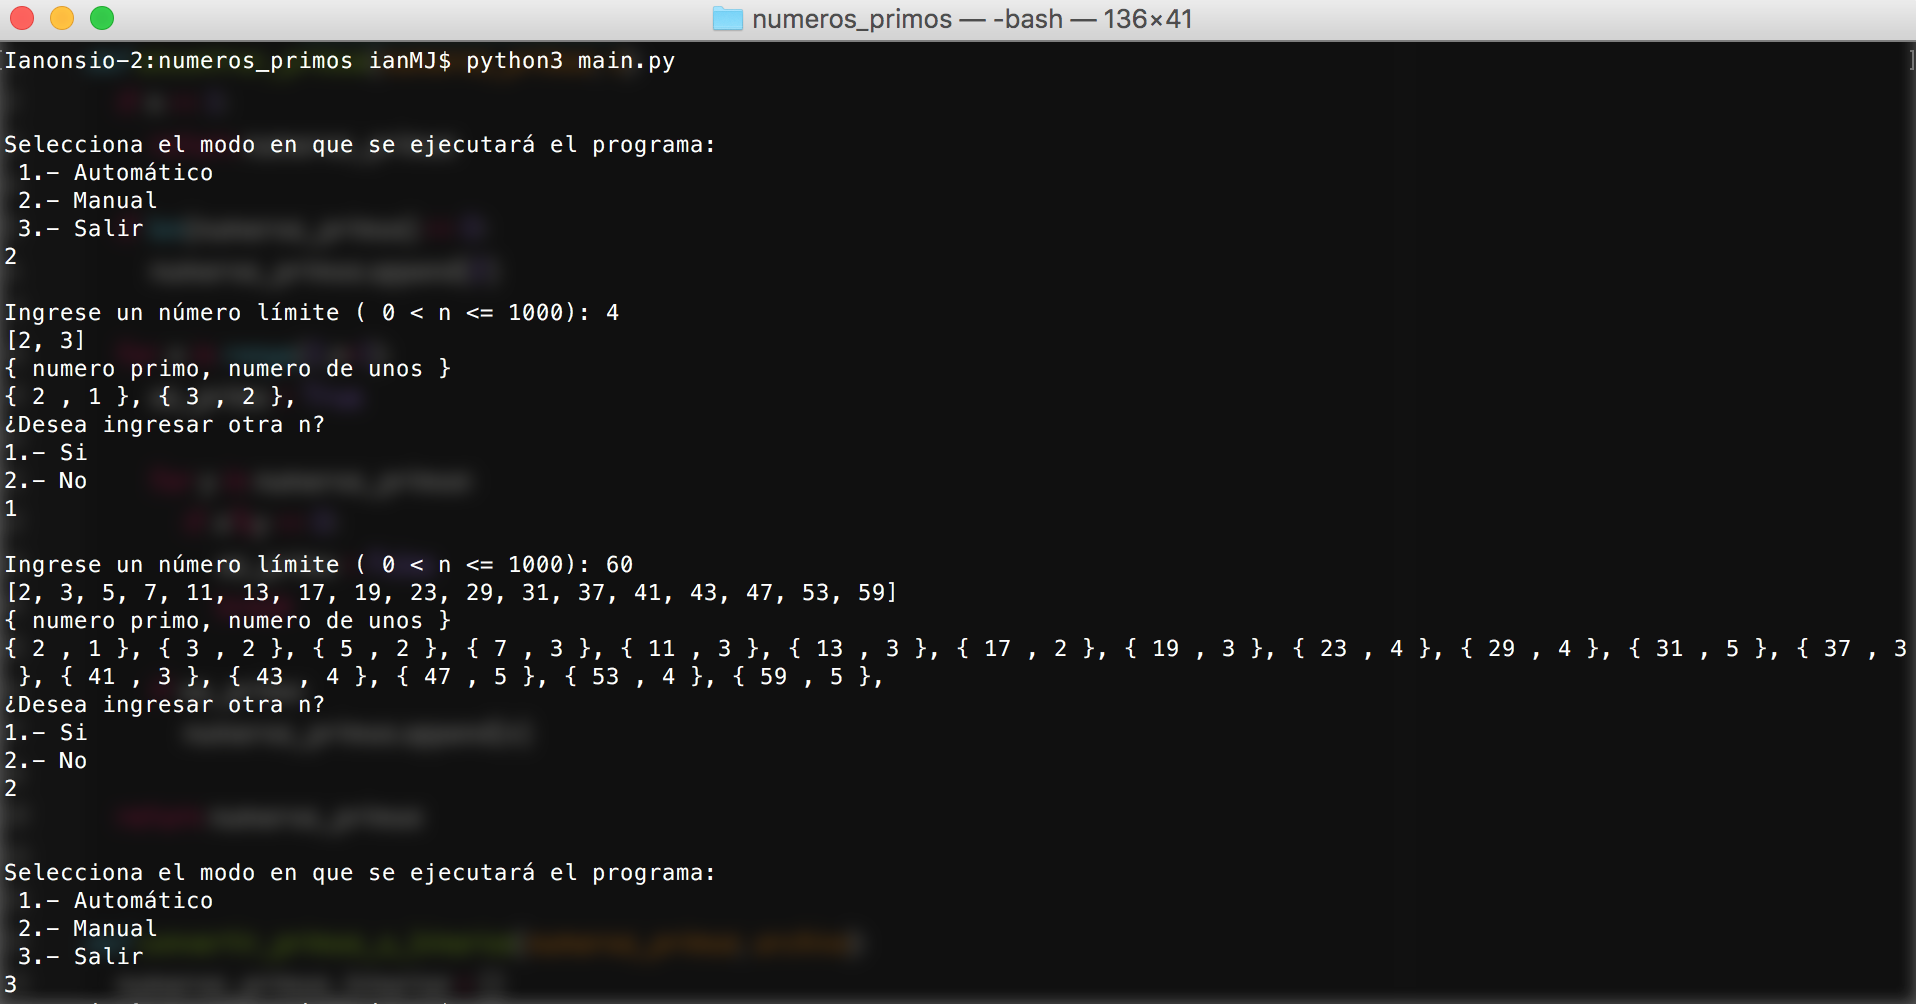
\includegraphics[width=\textwidth, height=9cm]{primos_manual}
\caption{El resultado de seleccionar la modalidad manual.}
\label{fig:primos_manual}
\end{figure}

\begin{figure}[H]
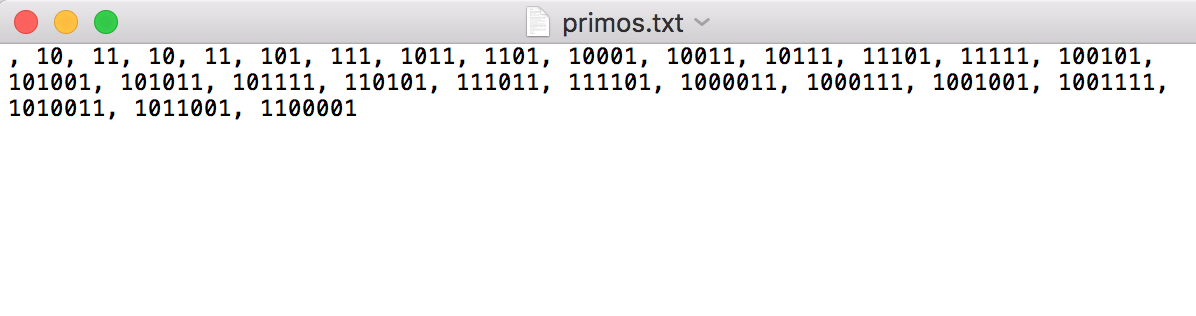
\includegraphics[width=\textwidth, height=5cm]{primos_manual_texto}
\caption{El resultado en texto de seleccionar la modalidad manual.}
\label{fig:primos_manual}
\end{figure}

\newpage

Se graficó la relación entre ceros y unos de los números primos cuando estos eran convertidos a binario. El resultado de evaluar un n = 1000, es el siguiente:
\begin{figure}[H]
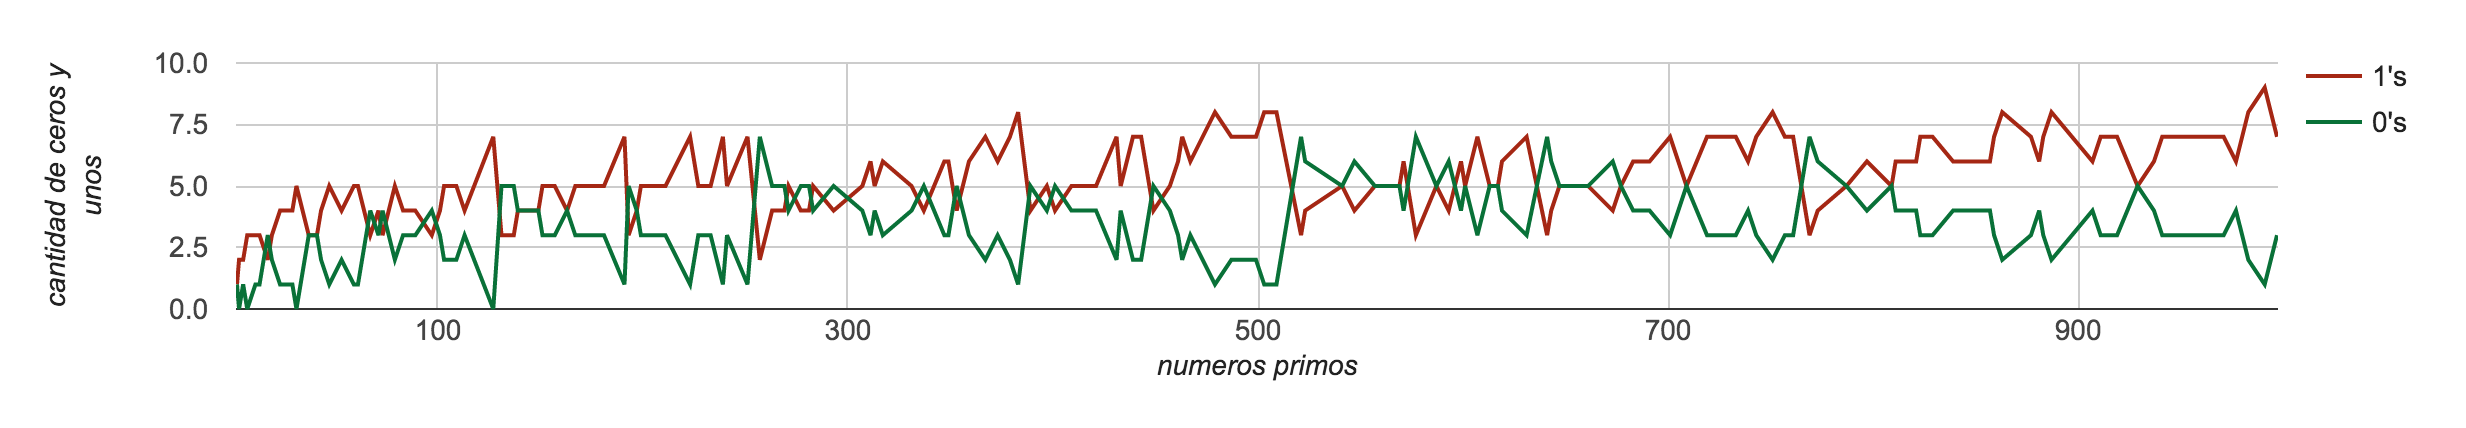
\includegraphics[width=\textwidth, height=5cm]{primos_grafica}
\caption{Gráfico de ceros y unos.}
\label{fig:primos_manual}
\end{figure}

%===============================================================================================
%===============================================================================================
%===============================================================================================
%===============================================================================================
%===============================================================================================
%===============================================================================================
%===============================================================================================

\newpage
\section{Palabras que terminan en ere}
Los autómatas son una forma de evaluar cadenas a través de una serie de estados. En concreto los autómatas determinísticos utilizan estados que solo pueden ser seguidos por otro estado. En esta sección se plantea un problema en el cual es muy conveniente utilizar un autómata para resolverlo y sirve como una introducción a esta teoría tan amplia.

\subsection{Descripción del problema}
Se tiene que elaborar un programa que pueda evaluar un texto y determinar cuales son las palabras que terminan con \textit{ere}. Además, deberá decir en que linea se encuentran. Para la realización de este programa, se debe de utilizar un autómata finito determinístico.


\subsection{Código}
El modelo del autómata utilizado para resolver este programa es el siguiente:

\begin{figure}[H]
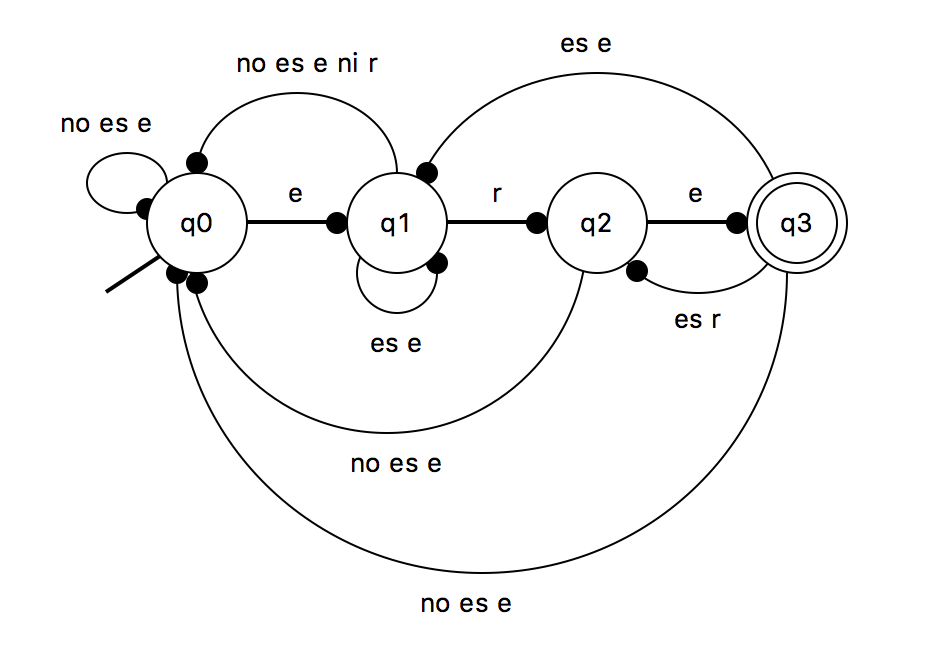
\includegraphics[width=\textwidth, height=10cm]{automata_ere}
\caption{El autómata utilizado para este problema.}
\label{fig:automata_ere_modelo}
\end{figure}

El lenguaje utilizado para este programa fue Python en su versión 3.5. El código para resolver el problema es el siguiente:\\

Archivo: main\_ere.py
\lstset{language=Python, breaklines=true, basicstyle=\footnotesize}
\begin{lstlisting}[frame=single]
from automata import obtener_palabras, graficar_automata
from ctypes import *

def main():
    seguir = True
    archivo = open('historial_ere.txt','w')
    archivo.close()
    while seguir:
        try:
            palabras_aceptadas = []
            texto = ""
            archivo = None

            opcion = imprimir_menu()

            if opcion == 1:
                while True:
                    print("\n\nIngrese un texto (dos veces la tecla enter para salir): \n")
                    tem = ''
                    t = ''
                    texto = []
                    contador = 0
                    while True:
                        t = input()
                        if t == '':
                            break
                        texto.append(t)

                    palabras_aceptadas = leer_texto(texto)
                    imprimir_palabras_aceptadas(palabras_aceptadas, opcion)

                    texto = input("\n\nDesea ingresar otra cosa? [s/n]: ")
                    if (texto != 's') and (texto != 'S'):
                        break

            elif opcion == 2:
                texto = input("\n\nIngrese el nombre de un archivo: \n")
                archivo = open(texto, "r")
                palabras_aceptadas = leer_texto(archivo)
                archivo.close()
                imprimir_palabras_aceptadas(palabras_aceptadas, opcion)
            elif opcion == 3:
                print("Sera utilizado el archivo heart.txt")
                archivo = open("heart.txt", "r")
                palabras_aceptadas = leer_texto(archivo)
                imprimir_palabras_aceptadas(palabras_aceptadas, opcion)
            elif opcion == 4:
                graficar_automata()
            else:
                return 0

        except Exception as e:
            print("Uuups!, parece que tuvimos un problema: ", e)
    return 1


def imprimir_menu():
    seguir = True
    while seguir:
        try:
            opcion = int(input("\n\nIngrese la opcion que desea: \n1.- Ingresar texto \n2.- Ingresar un archivo \n3.- Automatico \n4.- Ver grafico del automata \n5.- Salir\n"))
            return opcion
        except Exception as e:
            print("Por favor, ingrese un dato valido.")


def leer_texto(texto):
    aceptadas = None
    palabras_aceptadas = []
    contador = 1
    for linea in texto:
        aceptadas = obtener_palabras(linea)
        palabras_aceptadas.append([contador, aceptadas])
        contador += 1

    return palabras_aceptadas


def imprimir_palabras_aceptadas(palabras_aceptadas, seleccion):
    print("\n\n\n")
    contador = 0
    for x in palabras_aceptadas:
        if len(x[1]) > 0:
            print("")
            print("Linea ", str(x[0])+',', " palabras aceptadas: ", end=' ')
            for palabra in x[1]:
                print(palabra[0], '(No. palabra:'+str(palabra[1])+')', end=', ')


main()

\end{lstlisting}

\vspace{3em}

Archivo: automata\_ere.py
\lstset{language=Python, breaklines=true, basicstyle=\footnotesize}
\begin{lstlisting}[frame=single]
from tkinter import *
import time

def obtener_palabras(texto):
    archivo = open('historial_ere.txt','a')
    estado = 0
    palabras_aceptadas = []
    temporal = ''
    letra_auxiliar = ''
    ascii_axuliar = 0
    contador = 0
    estado_axiliar = ''
    for x in texto:
        letra_auxiliar = x
        letra_auxiliar = letra_auxiliar.lower()
        ascii_axuliar = ord(letra_auxiliar)
        if (ascii_axuliar >= 97 and ascii_axuliar <= 122) or (ascii_axuliar >= 224 and ascii_axuliar <= 255):
            print(letra_auxiliar)
            estado_axiliar = 'Delta(q'+str(estado)+', '+x+')-->'
            archivo.write(estado_axiliar)
            estado = automata(estado, letra_auxiliar)
            temporal += x
        else:
            contador += 1
            estado_axiliar = 'q'+str(estado)+'\n\n'
            archivo.write(estado_axiliar)
            if estado == 3:
                palabras_aceptadas.append([temporal, contador])
            temporal = ''
            estado = 0

    estado_axiliar = 'q'+str(estado)+'\n\n'
    archivo.write(estado_axiliar)
    archivo.close()
    print(estado)
    if estado == 3:
        contador += 1
        palabras_aceptadas.append([temporal, contador])

    return palabras_aceptadas


def automata(estado, letra_auxiliar):
    if estado == 0:
        return estado_cero(letra_auxiliar)
    elif estado == 1:
        return estado_uno(letra_auxiliar)
    elif estado == 2:
        return estado_dos(letra_auxiliar)
    elif estado == 3:
        return estado_tres(letra_auxiliar)
    else:
        return -1


def estado_cero(letra):
    if (ord(letra) >= 232 and ord(letra) <= 235) or letra == 'e':
        return 1
    else:
        return 0


def estado_uno(letra):
    if (ord(letra) >= 232 and ord(letra) <= 235) or letra == 'e':
        return 1
    elif letra == 'r':
        return 2
    else:
        return 0


def estado_dos(letra):
    if (ord(letra) >= 232 and ord(letra) <= 235) or letra == 'e':
        return 3
    else:
        return 0


def estado_tres(letra):
    if (ord(letra) >= 232 and ord(letra) <= 235) or letra == 'e':
        return 1
    elif letra == 'r':
        return 2
    else:
        return 0


def graficar_automata():
    raiz = Tk()
    raiz.title('Automata')
    raiz.geometry('500x350')
    canvas = Canvas(raiz, width=600, height=410, bg='white')
    canvas.place(x=0,y=0)
    canvas.pack(expand=YES, fill=BOTH)

    x = 90
    y = 100
    r = 50
    numero_circulos = 4
    opciones = ['e','r','e']
    canvas.create_line(x-20, y+r*1.2, x+.2*r, y+.8*r, width=2, fill='black')
    for i in range(numero_circulos):
        dibujos_especificos(canvas, i, x, y)
        x += r+50

    x = 90
    for i in range(numero_circulos):
        canvas.create_oval(x, y, x+r, y+r, width=1, fill='white')
        widget = Label(canvas, text='q'+str(i), fg='black', bg='white')
        widget.pack()
        canvas.create_window(x+.5*r, y+.5*r, window=widget)

        if i < numero_circulos-1:
            canvas.create_line(x+r, y+(r/2), x+r+50, y+(r/2), width=2, fill='black')
            widget = Label(canvas, text=opciones[i], fg='black', bg='white')
            widget.pack()
            canvas.create_window(x+r+25, y+(r/2)-15, window=widget)
            canvas.create_oval(x+r+40, y+(r/2)-5, x+r+50, y+(r/2)+5, width=1, fill='black')

        if i == numero_circulos -1:
            canvas.create_oval(x+5, y+5, x+r-5, y+r-5, width=1, fill='white')
        x += r+50

    raiz.mainloop()

def dibujos_especificos(canvas, i, x, y):
    if i == 0:
        xy = x+10, y-20, x+30, y+10
        canvas.create_oval(x-30,y-10, x+10,y+20, width=1)
        canvas.create_oval(x-5, y+13, x+5, y+23, width=1, fill='black')
        widget = Label(canvas, text='no es e', fg='black', bg='white')
        widget.pack()
        canvas.create_window(x-20, y-25, window=widget)
    elif i == 1:
        xy = x-75, y-40, x+25, y+40
        canvas.create_arc(xy, start=0, extent=180, style='arc')
        canvas.create_oval(x-80, y-10, x-70, y, width=1, fill='black')
        canvas.create_oval(x+5,y+30, x+45,y+70, width=1)
        widget = Label(canvas, text='no es e ni r', fg='black', bg='white')
        widget.pack()
        canvas.create_window(x-20, y-55, window=widget)
        canvas.create_oval(x+40,y+40, x+50,y+50, width=1, fill='black')
        widget = Label(canvas, text='es e', fg='black', bg='white')
        widget.pack()
        canvas.create_window(x+25, y+85, window=widget)
    elif i == 2:
        xy = x-180, y-70, x+20, y+130
        canvas.create_arc(xy, start=0, extent=-180, style='arc')
        widget = Label(canvas, text='no es e', fg='black', bg='white')
        widget.pack()
        canvas.create_window(x-75, y+145, window=widget)
        canvas.create_oval(x-180,y+50, x-170,y+60, width=1, fill='black')
    elif i == 3:
        xy = x-285, y-100, x+20, y+200
        canvas.create_arc(xy, start=0, extent=-180, style='arc')
        canvas.create_oval(x-290,y+45, x-280,y+55, width=1, fill='black')
        widget = Label(canvas, text='no es e', fg='black', bg='white')
        widget.pack()
        canvas.create_window(x-140, y+215, window=widget)
        xy = x-170, y+120, x+20, y-50
        canvas.create_arc(xy, start=0, extent=180, style='arc')
        canvas.create_oval(x-165,y+5, x-155,y-5, width=1, fill='black')
        widget = Label(canvas, text='es e', fg='black', bg='white')
        widget.pack()
        canvas.create_window(x-80, y-65, window=widget)
        xy = x-65, y, x+16, y+60
        canvas.create_arc(xy, start=0, extent=-180, style='arc')
        widget = Label(canvas, text='es r', fg='black', bg='white')
        widget.pack()
        canvas.create_window(x-24, y+73, window=widget)
        canvas.create_oval(x-60,y+44, x-50,y+54, width=1, fill='black')

\end{lstlisting}

\subsection{Pruebas}
Los siguientes, son los resultados que se obtuvieron del programa anterior.

\begin{figure}[H]
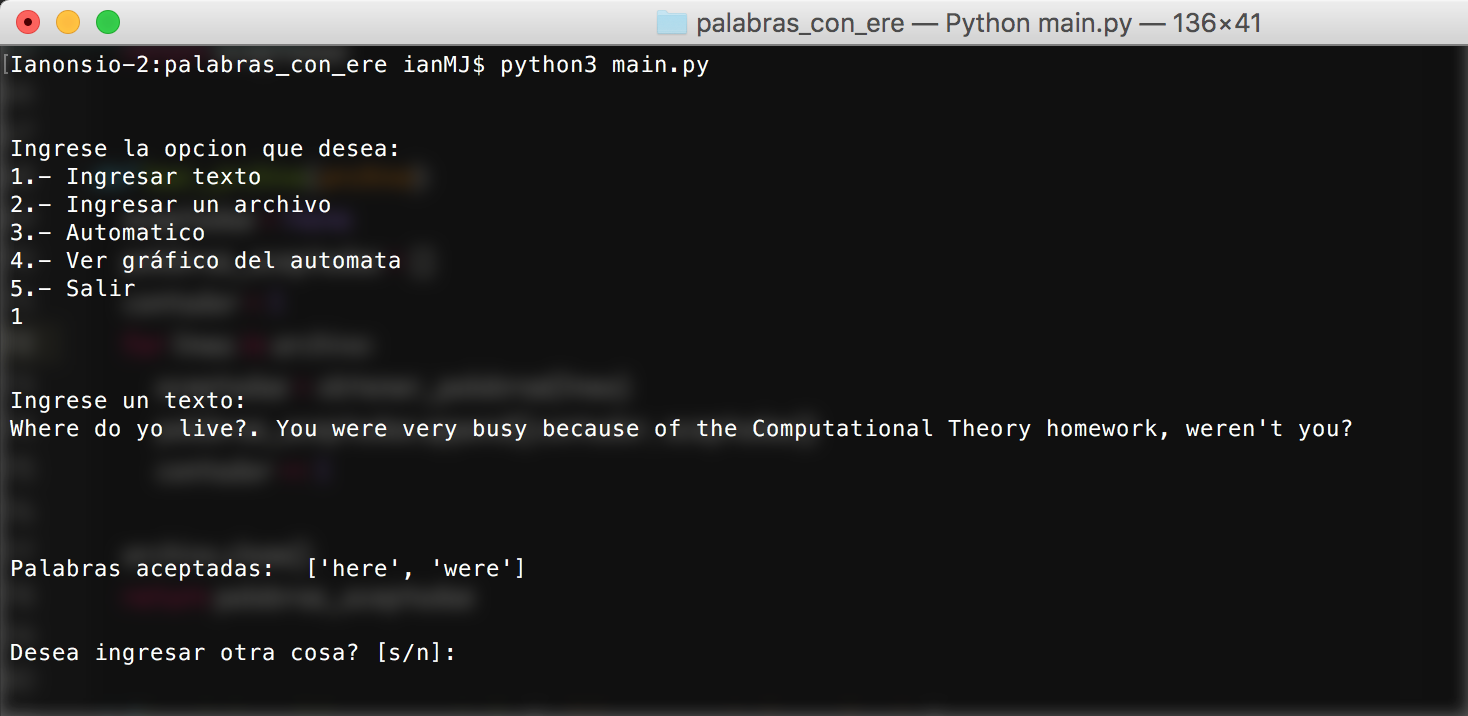
\includegraphics[width=\textwidth, height=8cm]{palabras_ere_texto}
\caption{Un texto ingresado de forma manual.}
\label{fig:automata_ere_texto}
\end{figure}

\begin{figure}[H]
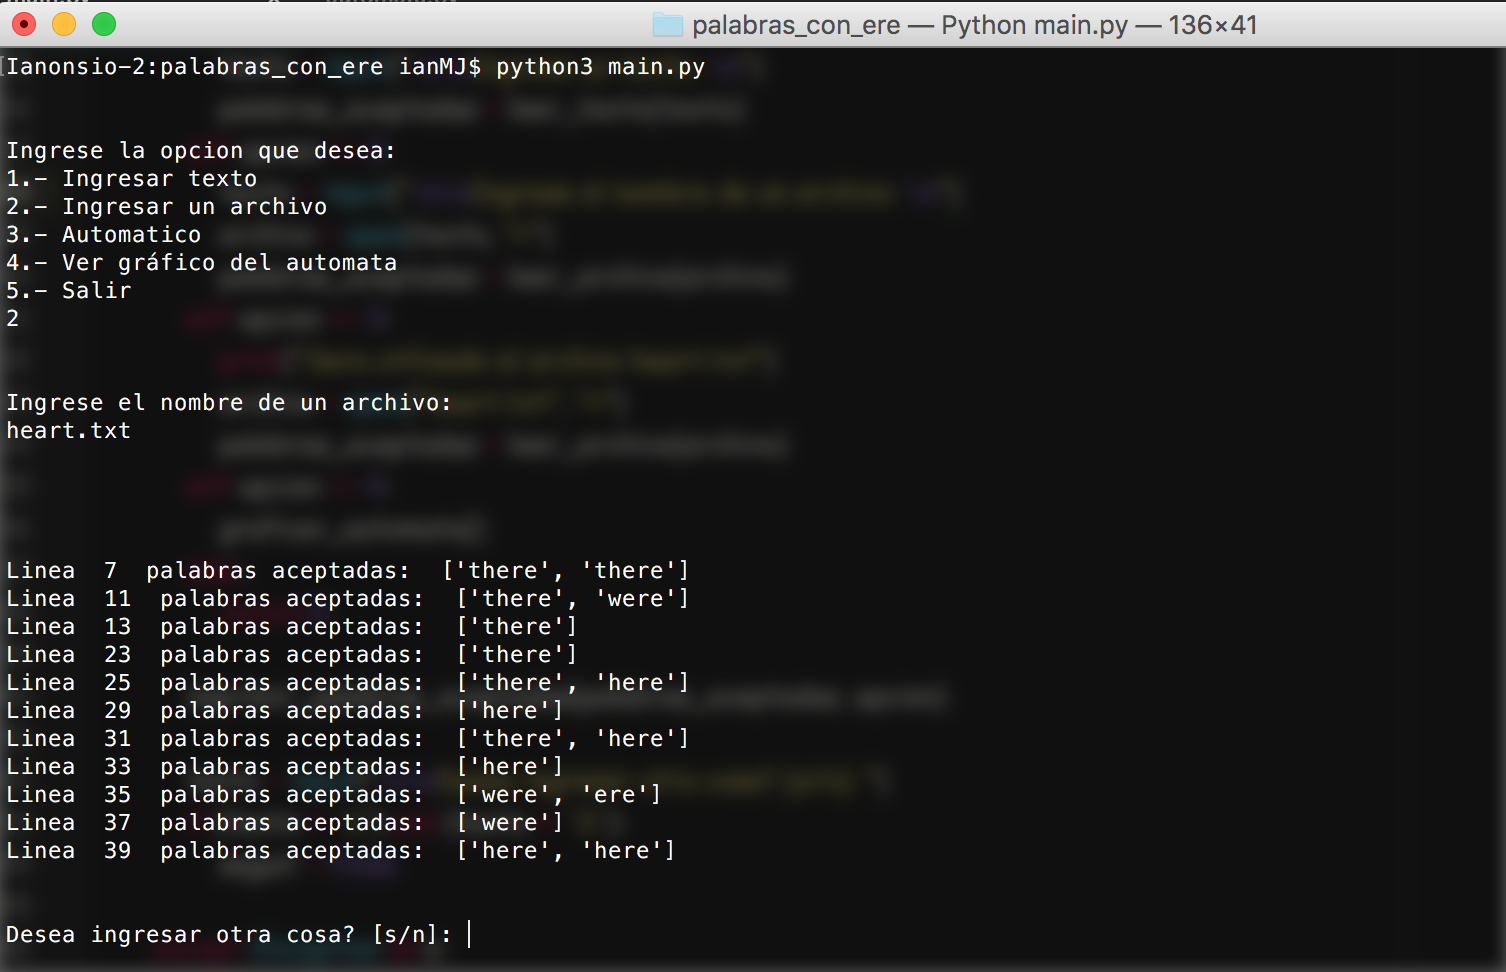
\includegraphics[width=\textwidth, height=8cm]{palabras_ere_archivo}
\caption{Un archivo ingresado de forma manual.}
\label{fig:automata_ere_archivo}
\end{figure}

\begin{figure}[H]
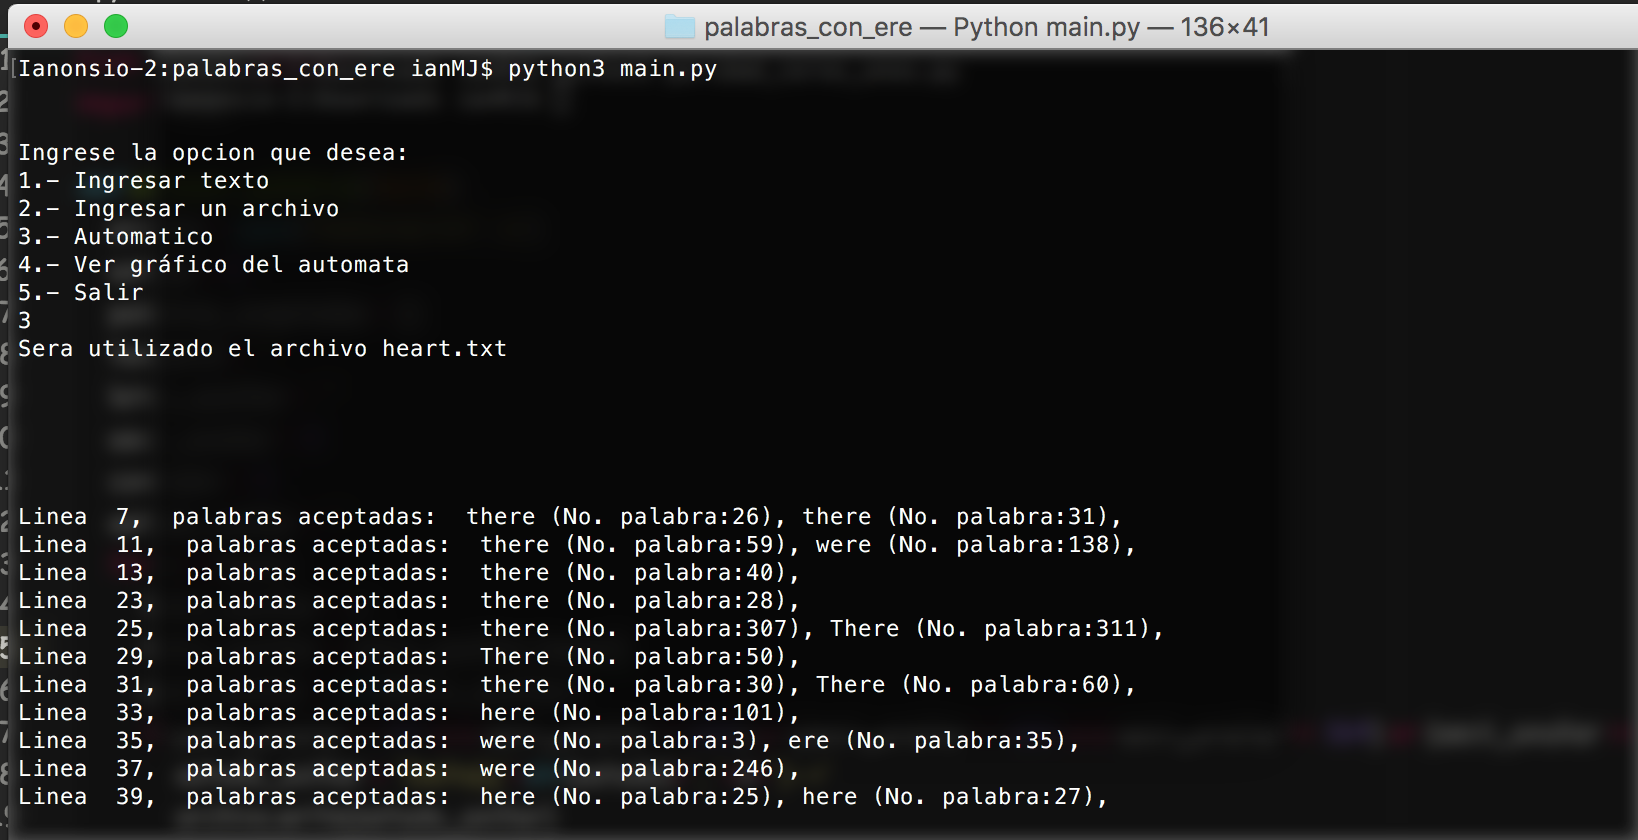
\includegraphics[width=\textwidth, height=8cm]{palabras_ere_auto}
\caption{Un archivo analizado de forma automática por el programa.}
\label{fig:automata_ere_auto}
\end{figure}

\begin{figure}[H]
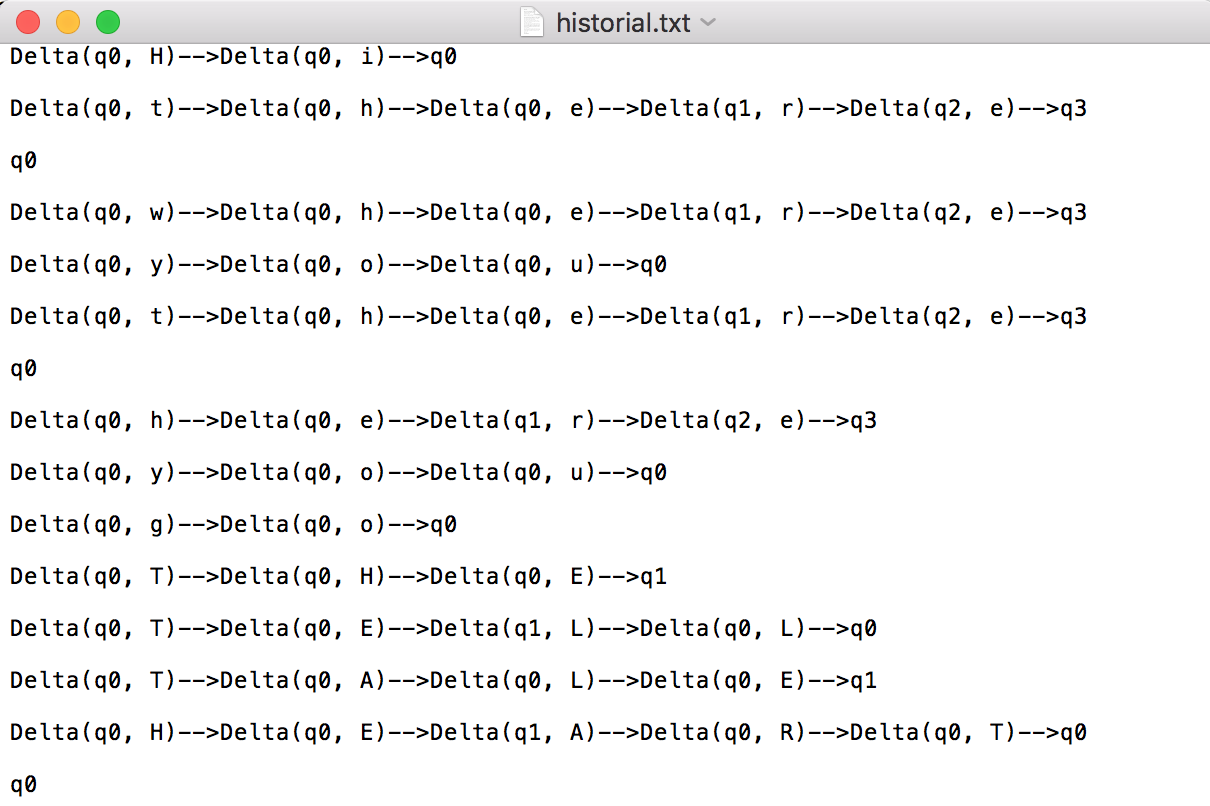
\includegraphics[width=\textwidth, height=8cm]{palabras_ere_historial}
\caption{El historial del programa.}
\label{fig:automata_ere_auto}
\end{figure}

\begin{figure}[H]
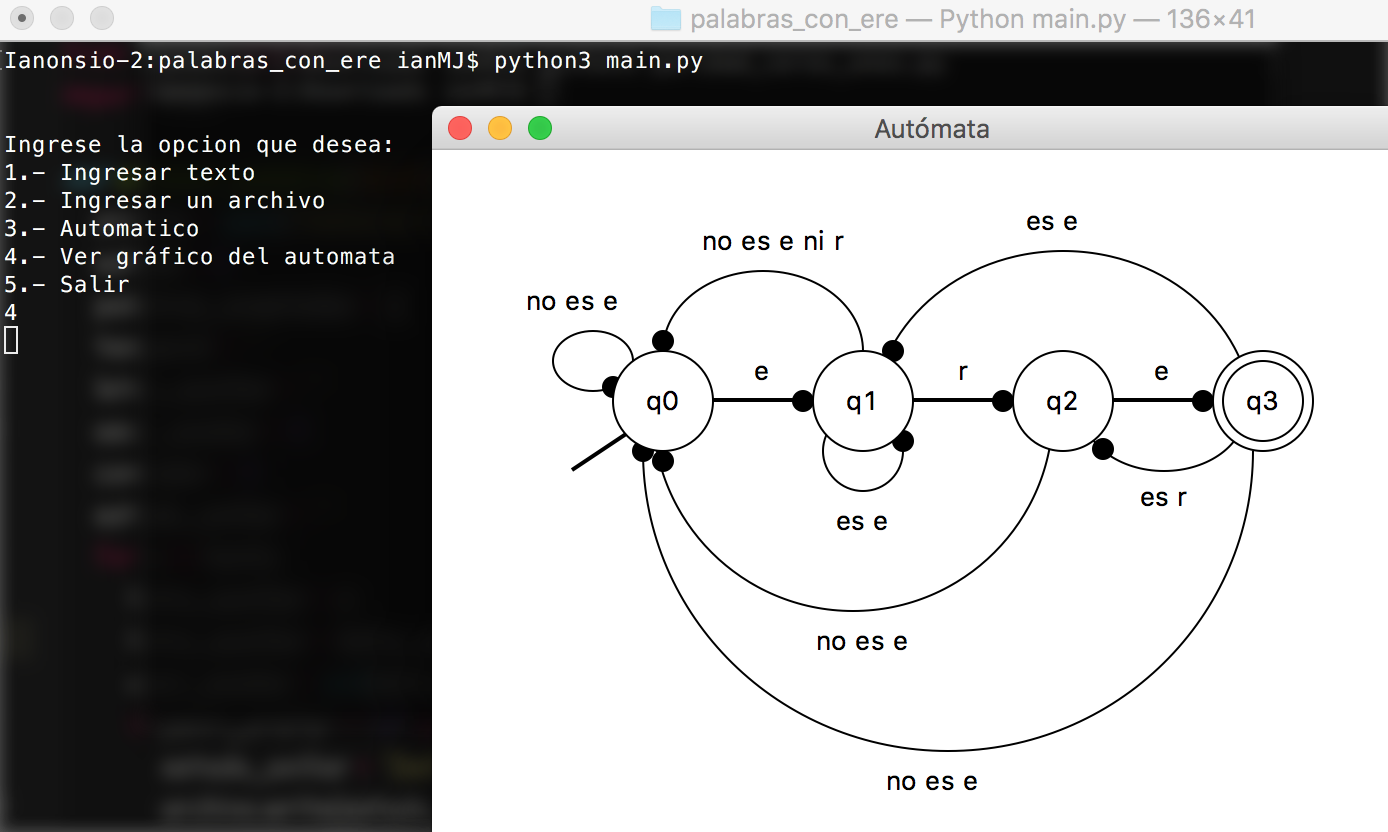
\includegraphics[width=\textwidth, height=8cm]{automata_prueba}
\caption{El programa imprimiendo el autómata.}
\label{fig:automata_ere_prueba}
\end{figure}

%===============================================================================================
%===============================================================================================
%===============================================================================================
%===============================================================================================
%===============================================================================================
%===============================================================================================
%===============================================================================================


\newpage
\section{Paridad de ceros y unos}
Los autómatas, son una manera de poder evaluar cadenas y determinar si cumplen con ciertas características que nosotros deseamos. En este caso se plantea un problema para practicar esta funcionalidad.

\subsection{Descripción del problema}
Se tiene que crear un programa que determine si una cadena de números binarios tiene una cantidad par de ceros y de unos. Para la resolución de este problema, se tiene que utilizar un autómata finito determinístico.

\subsection{Código}
El modelo de autómata que se utilizo para resolver este problema es el siguiente:

\begin{figure}[H]
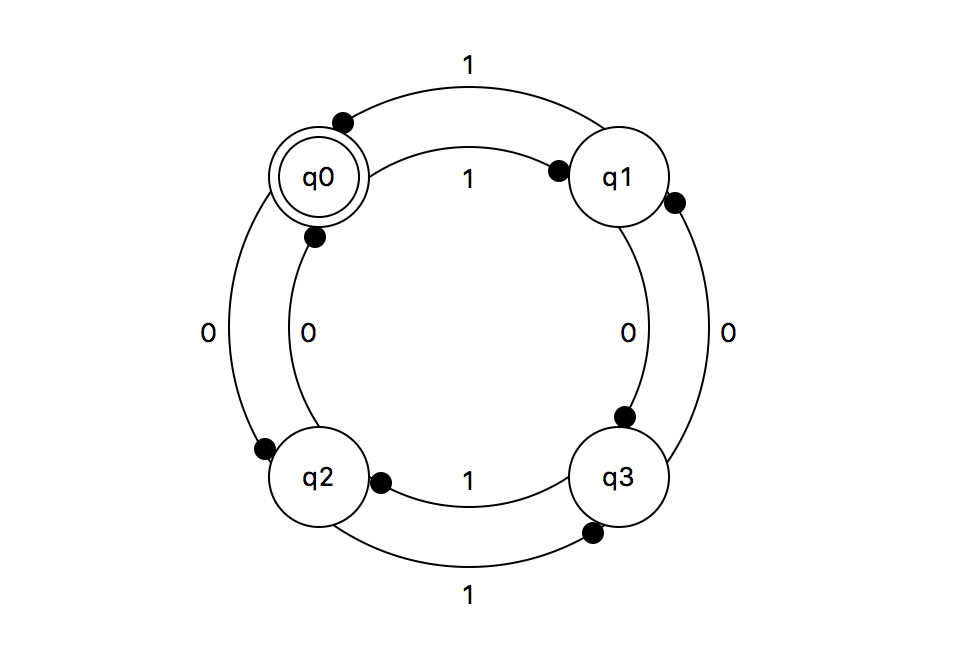
\includegraphics[width=\textwidth, height=10cm]{automata_paridad}
\caption{El autómata utilizado para este problema.}
\label{fig:automata_paridad_modelo}
\end{figure}

El lenguaje utilizado para este programa fue Python en su versión 3.5. El código para resolver el problema es el siguiente:\\

Archivo: main\_paridad.py
\lstset{language=Python, breaklines=true, basicstyle=\footnotesize}
\begin{lstlisting}[frame=single]
from metodos import obtener_paridades, ejecuta_diagrama
from random import random

def main():
    archivo = open("historial_paridad.txt","w")
    try:
        while True:
            opcion = imprimir_menu()

            if opcion == 1:
                ejecuta_manual()
            elif opcion == 2:
                ejecuta_automatico()
            elif opcion == 3:
                ejecuta_diagrama()
            else:
                return 1

    except Exception as e:
        print('Uuups, parece que hubo un problema: ',e)




def ejecuta_manual():
    while True:
        texto = input('\n\nIntrodusca un numero binario: ')
        es_permitida = obtener_paridades(texto)
        opcion = ''

        if es_permitida:
            print('La palabra ', texto, ' es permitida')
        else:
            print('La palabra ', texto, ' no es permitida')

        opcion = input("Quiere ingresar otro numero? [s/n]  ")
        if opcion != 's' and opcion != 'S':
            return 1



def ejecuta_automatico():
    limite = 0
    aleatorio = 0
    numero = ''
    i = 0
    seguir = True
    es_permitida = False
    continuar = 0

    while seguir:
        limite = int(random() * 2000) % 1001
        i = 0
        while i < limite:
            aleatorio = int(random() * 10) % 2
            if aleatorio == 0:
                numero += '0'
            else:
                numero += '1'
            i += 1

        print('\n\nSe utilizara la palabra: ', numero)
        es_permitida = obtener_paridades(numero)
        if es_permitida:
            print('La palabra ', numero, ' es permitida')
        else:
            print('La palabra ', numero, ' no es permitida')

        continuar = int(random() * 10) % 2
        if continuar == 0:
            seguir = False
        else:
            seguir = True


def imprimir_menu():
    while True:
        try:
            opcion = int(input("\n\n\nEscoja lo que desea: \n1.- Manual \n2.- Automatico \n3.- Ver diagrama \n4.- Salir\n\n"))
            if opcion >= 1 and opcion <= 4:
                return opcion
            else:
                raise Exception
        except Exception as e:
            print('Por favor, intrudusca un dato valido')


main()

\end{lstlisting}

\vspace{1em}

Archivo: metodos\_paridad.py
\lstset{language=Python, breaklines=true, basicstyle=\footnotesize}
\begin{lstlisting}[frame=single]
from tkinter import *

def obtener_paridades(texto):
    archivo = open("historial_paridad.txt", 'a')
    historial = ''
    palabras_permitidas = []
    temporal = ''
    estado = 0
    for x in texto:
        historial = '(q'+str(estado)+', '+x+')-->'
        print(historial, end='')
        archivo.write(historial)
        estado = automata(estado, x)

    historial = 'q'+str(estado)
    print(historial, end='  ')
    archivo.write(historial)
    archivo.write('\n')
    archivo.close()
    if estado == 0:
        return True
    else:
        return False


def automata(estado, letra):
    if estado == 0:
        return estado_cero(letra)
    elif estado == 1:
        return estado_uno(letra)
    elif estado == 2:
        return estado_dos(letra)
    else:
        return estado_tres(letra)


def estado_cero(letra):
    if letra == '1':
        return 1
    elif letra == '0':
        return 2
    else:
        return -1


def estado_uno(letra):
    if letra == '1':
        return 0
    elif letra == '0':
        return 3
    else:
        return -1


def estado_dos(letra):
    if letra == '1':
        return 3
    elif letra == '0':
        return 0
    else:
        return -1


def estado_tres(letra):
    if letra == '1':
        return 2
    elif letra == '0':
        return 1
    else:
        return -1

def ejecuta_diagrama():
    ventana = Tk()
    ventana.title("Automata")
    ventana.geometry("500x350")
    canvas = Canvas(ventana, width=600, height=410, bg='white')
    canvas.place(x=0,y=0)
    canvas.pack(expand=YES, fill=BOTH)

    x = 140
    y = 70
    r = 50

    dibujos_especificos(x,y, canvas, r)


    for i in range(2):
        canvas.create_oval(x, y, x+r, y+r, width=1, fill="white")
        canvas.create_oval(x, y+r+100, x+r, y+2*r+100, width=1, fill="white")

        widget = Label(canvas, text='q'+str(i), fg='black', bg='white')
        widget.pack()
        canvas.create_window(x+25, y+(r/2), window=widget)

        widget = Label(canvas, text='q'+str(i+2), fg='black', bg='white')
        widget.pack()
        canvas.create_window(x+25, y+2*r+75, window=widget)

        if i == 0:
            canvas.create_oval(x+5, y+5, x+r-5, y+r-5, width=1)

        x += r + 100

    ventana.mainloop()


def dibujos_especificos(x, y, canvas, r):
        canvas.create_oval(x-20, y-20, x+r+170, y+2*r+120)
        canvas.create_oval(x+10, y+10, x+r+140, y+2*r+90)

        canvas.create_oval(x+32, y-7, x+42, y+3, width=1, fill="black")
        canvas.create_oval(x+140, y+17, x+150, y+27, width=1, fill="black")
        canvas.create_oval(x+173, y+140, x+183, y+150, width=1, fill="black")
        canvas.create_oval(x+50.5, y+173, x+60.5, y+183, width=1, fill="black")
        canvas.create_oval(x+17.5, y+50, x+27.5, y+60, width=1, fill="black")
        canvas.create_oval(x-7.3, y+156, x+2.7, y+166, width=1, fill="black")
        canvas.create_oval(x+156.5, y+198, x+166.5, y+208, width=1, fill="black")
        canvas.create_oval(x+197.5, y+33, x+207.5, y+43, width=1, fill="black")

        widget = Label(canvas, text='1', fg='black', bg='white')
        widget.pack()
        canvas.create_window(x+100, y-31, window=widget)
        widget = Label(canvas, text='1', fg='black', bg='white')
        widget.pack()
        canvas.create_window(x+100, y+26, window=widget)

        widget = Label(canvas, text='1', fg='black', bg='white')
        widget.pack()
        canvas.create_window(x+100, y+177, window=widget)
        widget = Label(canvas, text='1', fg='black', bg='white')
        widget.pack()
        canvas.create_window(x+100, y+234, window=widget)

        widget = Label(canvas, text='0', fg='black', bg='white')
        widget.pack()
        canvas.create_window(x-30, y+103, window=widget)
        widget = Label(canvas, text='0', fg='black', bg='white')
        widget.pack()
        canvas.create_window(x+20, y+103, window=widget)

        widget = Label(canvas, text='0', fg='black', bg='white')
        widget.pack()
        canvas.create_window(x+180, y+103, window=widget)
        widget = Label(canvas, text='0', fg='black', bg='white')
        widget.pack()
        canvas.create_window(x+230, y+103, window=widget)

\end{lstlisting}

\newpage
\subsection{Pruebas}
A continuación se presentan imágenes de los resultados del programa corriendo:

\begin{figure}[H]
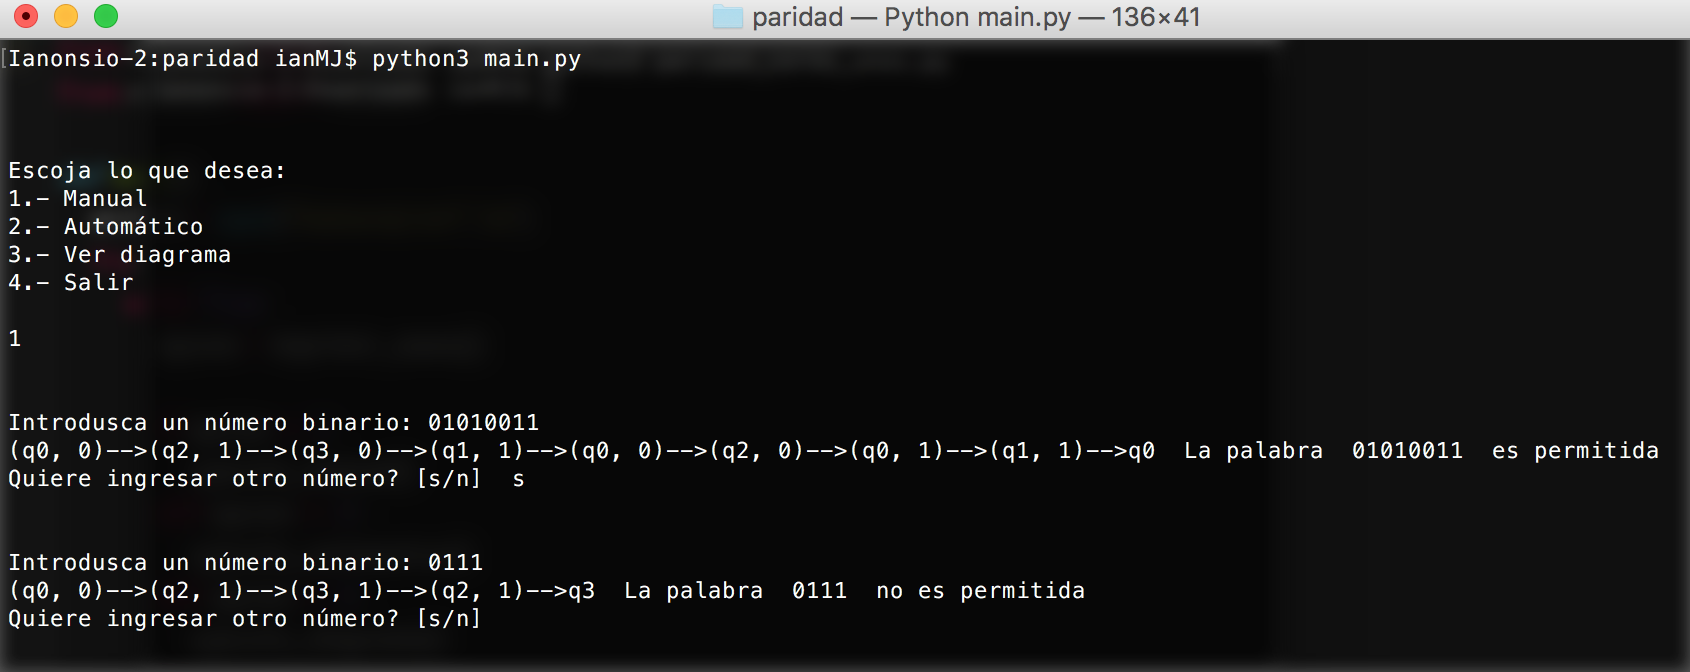
\includegraphics[width=\textwidth, height=8cm]{paridad_manual}
\caption{Números ingresados manualmente.}
\label{fig:automata_paridad_texto}
\end{figure}

\begin{figure}[H]
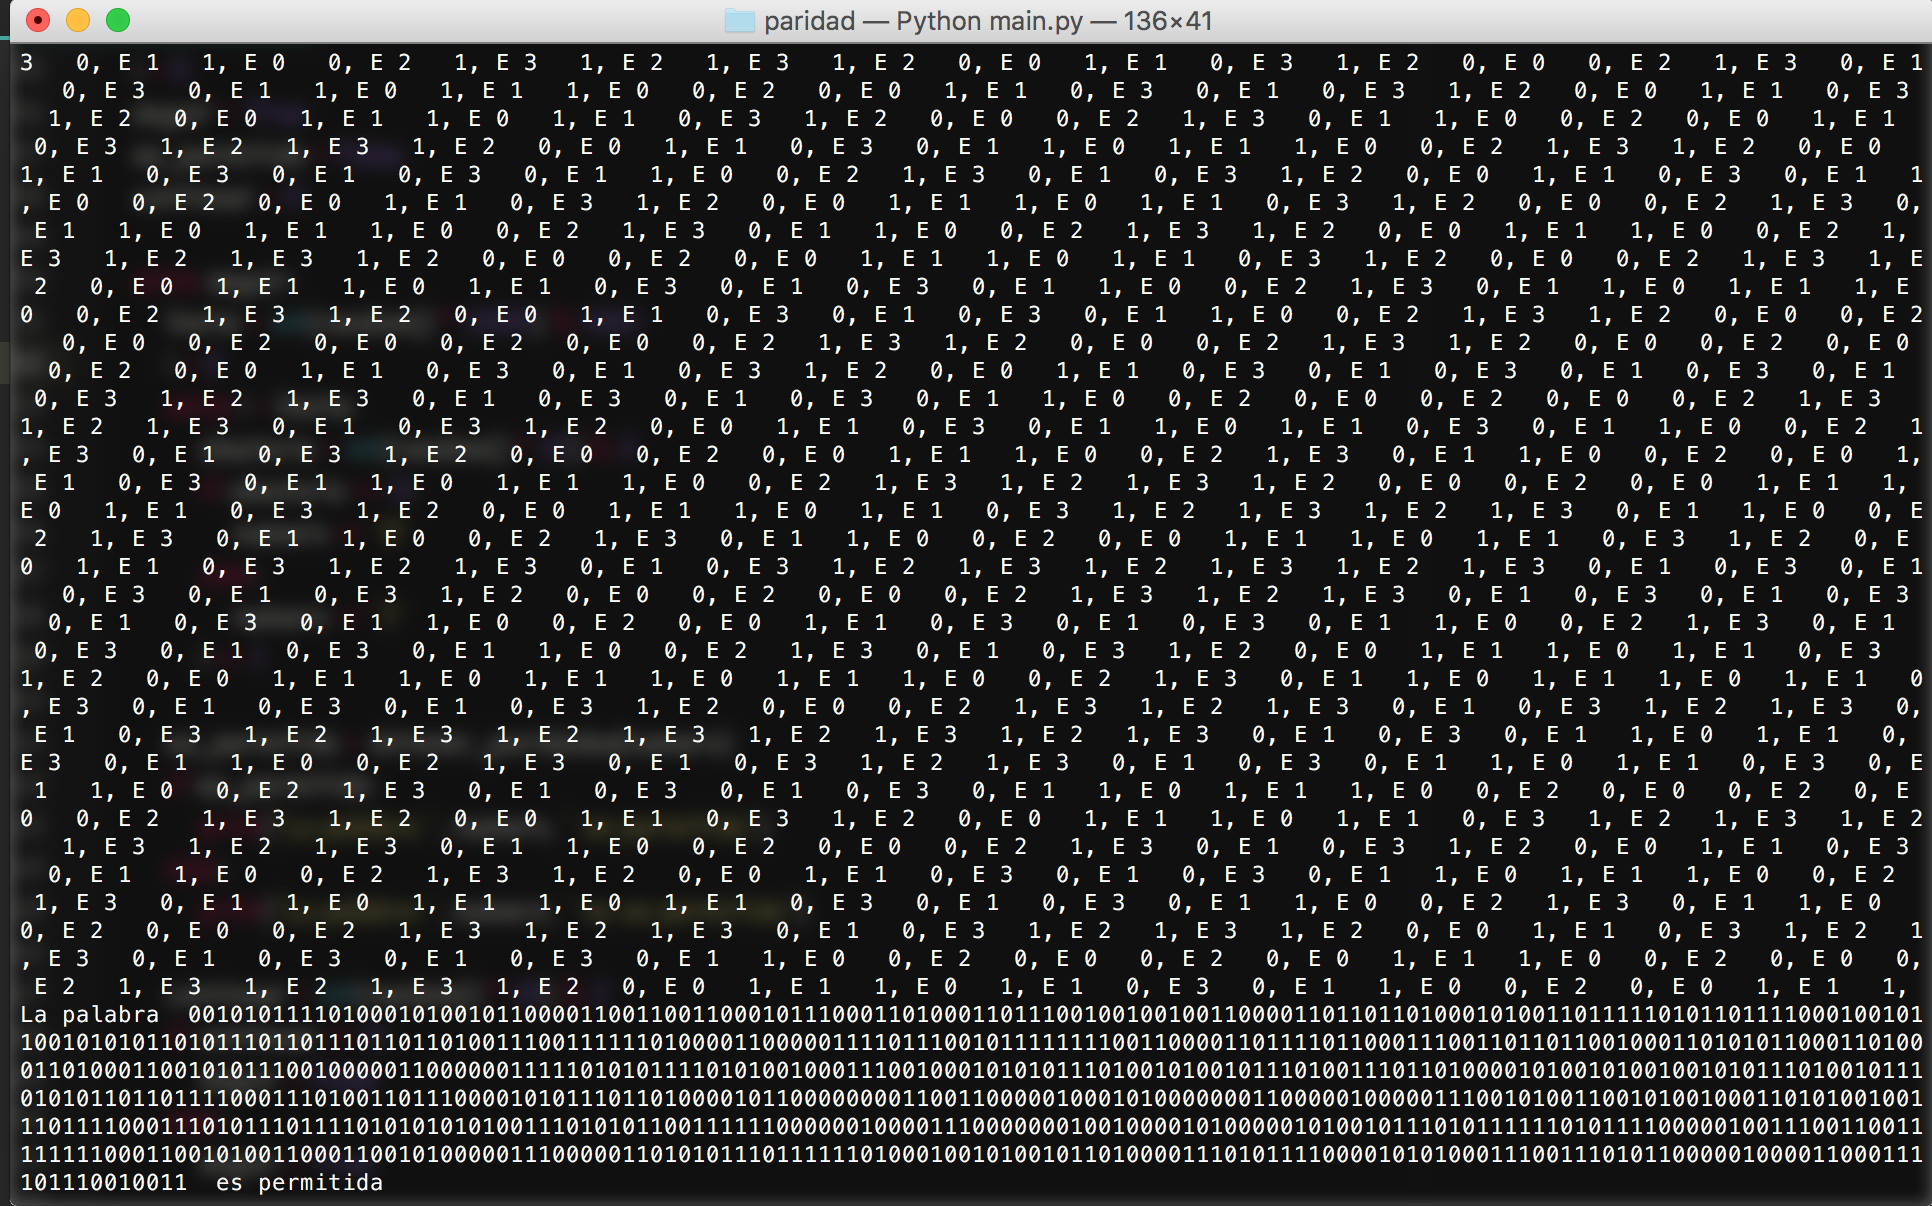
\includegraphics[width=\textwidth, height=8cm]{paridad_auto}
\caption{Modo automático.}
\label{fig:automata_paridad_auto}
\end{figure}

\begin{figure}[H]
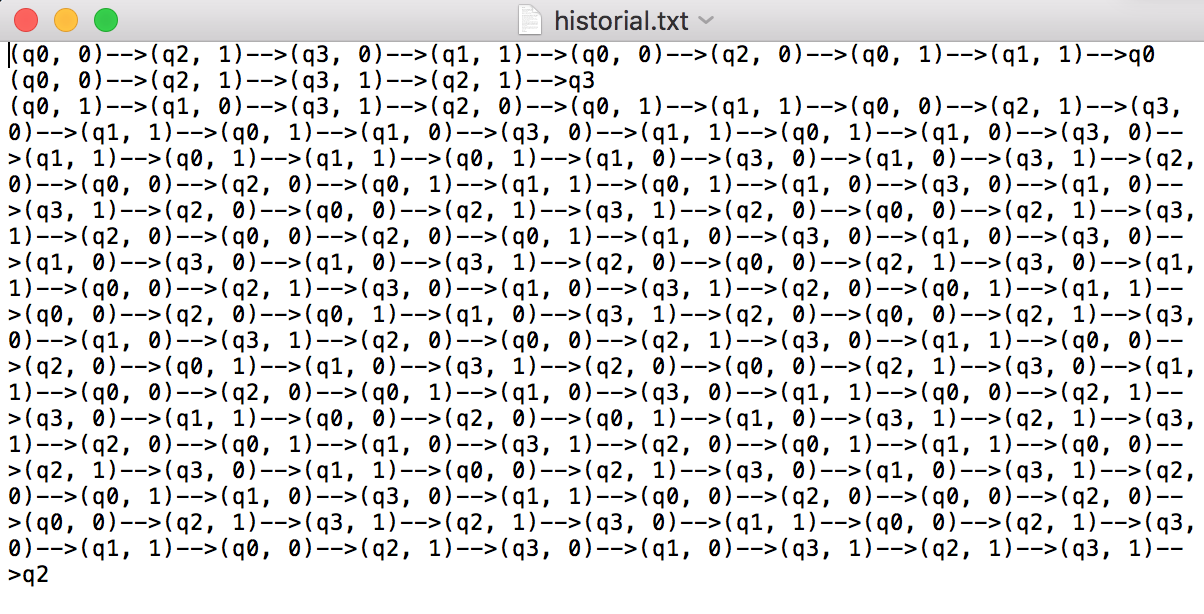
\includegraphics[width=\textwidth, height=8cm]{paridad_historial}
\caption{El historial del programa.}
\label{fig:automata_ere_auto}
\end{figure}

\begin{figure}[H]
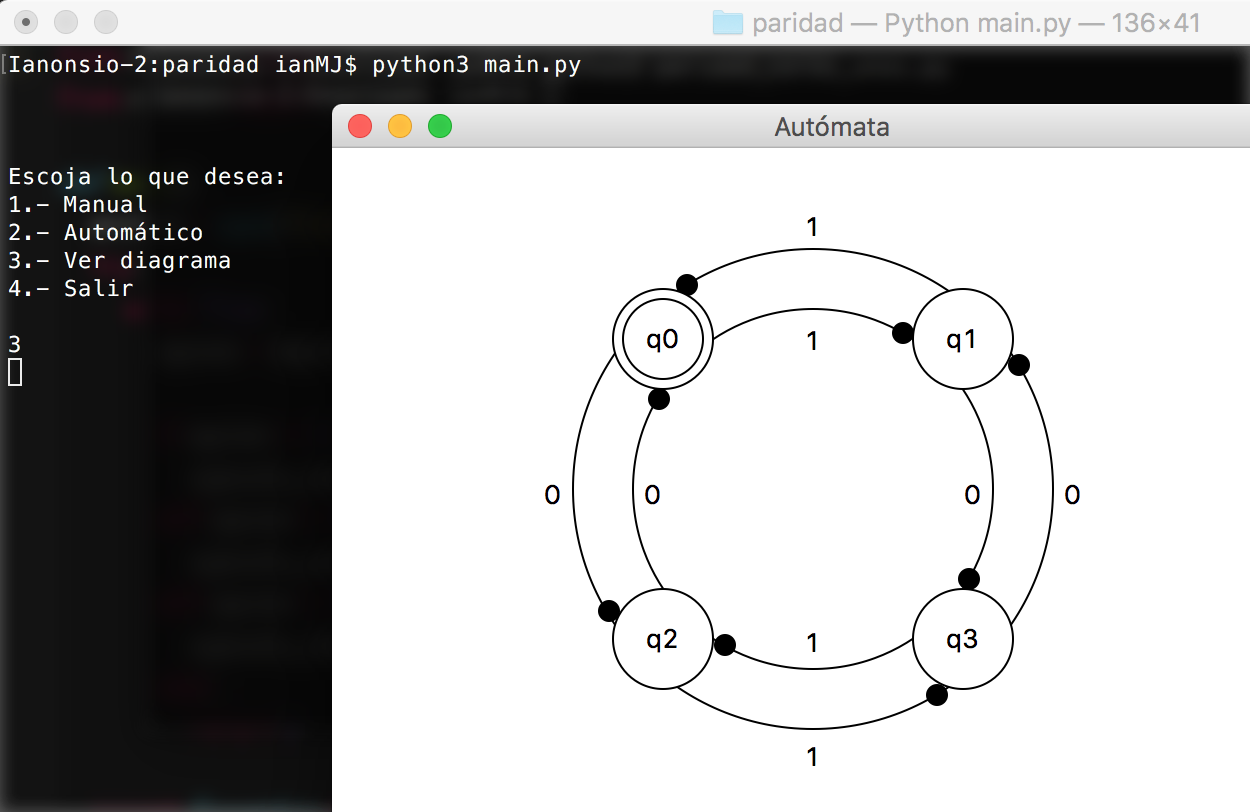
\includegraphics[width=\textwidth, height=8cm]{automata_paridad_prueba}
\caption{El programa imprimiendo el autómata.}
\label{fig:automata_paridad_prueba}
\end{figure}

%===============================================================================================
%===============================================================================================
%===============================================================================================
%===============================================================================================
%===============================================================================================
%===============================================================================================
%===============================================================================================

\newpage
\section{Protocolo}
Un protocolo es una serie de reglas para facilitar un fin. En este caso se presenta un ejemplo de un bosquejo de un protocolo para la transferencia de datos utilizando autómatas.

\subsection{Descripción del problema}
Se necesita crear un programa que genere 50 cadenas aleatoriamente para que después de tres segundos, que sería un tiempo de espera suficiente en este caso, comience a filtrar las cadenas que son validas de acuerdo a un criterio establecido. Para este problema, el criterio sera la paridad de ceros y unos, exactamente el mismo autómata de la sección anterior.

\subsection{Código}
El diagrama del protocolo es el siguiente \cite{stanford}

\begin{figure}[H]
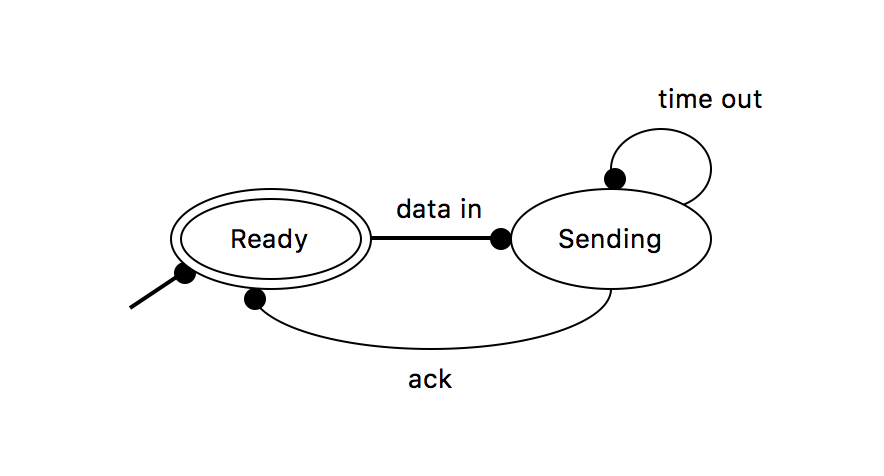
\includegraphics[width=\textwidth, height=10cm]{automata_protocolo}
\caption{El autómata utilizado para este problema.}
\label{fig:automata_protocolo_modelo}
\end{figure}

El lenguaje utilizado para este programa fue Python en su versión 3.5. El código para resolver el problema es el siguiente:\\

Archivo: main\_protocolo.py
\lstset{language=Python, breaklines=true, basicstyle=\footnotesize}
\begin{lstlisting}[frame=single]
from protocolo import *
from grafico_automata import dibujar_grafico_automata
from random import random


def main():
    try:
        while True:
            opcion = imprimir_menu()

            if opcion == 1:
                nombre_archivo = "palabras_generadas.txt"
                archivo = open(nombre_archivo, 'w')
                archivo.close()

                while True:
                    estado_encendido = int(random() * 100) % 3
                    estado = 0
                    if estado_encendido == 1:
                        print('\nEstado de la maquina: Encendido')
                    else:
                        print('\nEstado de la maquina: Apagado')
                        return 1
                    while True:
                        estado = automata_protocolo(estado)
                        if estado == 0:
                            break
            elif opcion == 2:
                dibujar_grafico_automata()
            else:
                return 1


    except Exception as e:
        print('Uuups, parece que hubo un problema: ',e)


def imprimir_menu():
    seguir = True
    while seguir:
        try:
            opcion = int(input("\n\nIngrese la opcion que desea: \n1.- Iniciar \n2.- Ver grafico \n3.- Salir \n"))
            return opcion
        except Exception as e:
            print("Por favor, ingrese un dato valido.")


main()

\end{lstlisting}

\vspace{1em}

Archivo: protocolo.py
\lstset{language=Python, breaklines=true, basicstyle=\footnotesize}
\begin{lstlisting}[frame=single]
from random import random
import time
from tkinter import *

def automata_protocolo(estado):
    if estado == 0:
        return crear_palabras()
    elif estado == 1:
        return enviar_datos()
    else:
        return -1


def enviar_datos():
    retrazar(3)
    return evaluar('palabras_generadas.txt')


def crear_palabras():
    nombre_archivo = 'palabras_generadas.txt'
    archivo = open(nombre_archivo, "a")
    longitud = 32
    aleatorio_numero = 0
    for x in range(0,  50):
        i = 0
        par = int(random() * 10) % 2
        while  i < longitud:
            aleatorio_numero = int(random() * 10) % 2
            if par == 0:
                archivo.write(str(aleatorio_numero)*2)
                i += 2
            else:
                archivo.write(str(aleatorio_numero))
                i += 1
        archivo.write(" ")
    archivo.close()

    return 1

def retrazar(tiempo):
    time.sleep(tiempo)


def evaluar(nombre_archivo):
    archivo = open(nombre_archivo, 'r')
    aceptadas = open("palabras_aceptadas.txt", "w")
    historial = open("historial_protocolo.txt", "w")
    historial_auxiliar = ''
    palabras_permitidas = []
    temporal = ''
    estado = 0
    letra = ''
    while True:
        letra = archivo.read(1)
        if not letra:
            break

        if letra != ' ':
            historial_auxiliar = 'Delta(q'+str(estado)+', '+letra+')-->'
            estado = automata(estado, letra)
            temporal += letra
        else:
            historial_auxiliar = 'q'+str(estado)+'\n\n\n'
            if estado == 0:
                palabras_permitidas.append(temporal)
                aceptadas.write(temporal)
                aceptadas.write('\n')
            estado = 0
            temporal = ''

        historial.write(historial_auxiliar)

    archivo.close()
    aceptadas.close()
    historial.close()
    print("Palabras aceptadas:\n" ,palabras_permitidas)
    return 0

def automata(estado, x):
    if estado == 0:
        return estado_cero(x)
    elif estado == 1:
        return estado_uno(x)
    elif estado == 2:
        return estado_dos(x)
    elif estado == 3:
        return estado_tres(x)
    else:
        return -1



def estado_cero(letra):
    if letra == '1':
        return 1
    elif letra == '0':
        return 2
    else:
        return -1


def estado_uno(letra):
    if letra == '1':
        return 0
    elif letra == '0':
        return 3
    else:
        return -1


def estado_dos(letra):
    if letra == '1':
        return 3
    elif letra == '0':
        return 0
    else:
        return -1


def estado_tres(letra):
    if letra == '1':
        return 2
    elif letra == '0':
        return 1
    else:
        return -1

\end{lstlisting}

\vspace{1em}

Archivo: grafico\_automata\_protocolo.py
\lstset{language=Python, breaklines=true, basicstyle=\footnotesize}
\begin{lstlisting}[frame=single]
from tkinter import *

def dibujar_grafico_automata():
    raiz = Tk()
    raiz.title('Automata')
    raiz.geometry('450x250')
    canvas = Canvas(raiz, width=600, height=410, bg='white')
    canvas.place(x=0,y=0)
    canvas.pack(expand=YES, fill=BOTH)

    x = 90
    y = 100
    r = 50
    numero_circulos = 2
    opciones = ['Ready', 'Sending']
    canvas.create_line(x-20, y+r*1.2, x+.2*r, y+.8*r, width=2, fill='black')
    canvas.create_oval(x+.2*r - 8, y+.8*r +7, x+.2*r +2 , y+.8*r-3, width=1, fill='black')

    for i in range(numero_circulos):
        if i == 1:
            canvas.create_oval(x+r, y+10, x+2*r, y-30, width=1, fill='white')
            canvas.create_oval(x+r-3, y-10, x+r+7, y, width=1, fill='black')
            widget = Label(canvas, text='time out', fg='black', bg='white')
            widget.pack()
            canvas.create_window(x+2*r, y-r+5, window=widget)
            xy = x-2*r-30, y+80, x+r, y+r-30
            canvas.create_arc(xy, start=0, extent=-180, style='arc')
            widget = Label(canvas, text='ack', fg='black', bg='white')
            widget.pack()
            canvas.create_window(x-r+10, y+95, window=widget)
            canvas.create_oval(x-2*r-33, y+50, x-2*r-23, y+60, width=1, fill='black')


        canvas.create_oval(x, y, x+2*r, y+r, width=1, fill='white')
        widget = Label(canvas, text=opciones[i], fg='black', bg='white')
        widget.pack()
        canvas.create_window(x+r, y+.5*r, window=widget)

        if i < numero_circulos-1:
            canvas.create_line(x+2*r, y+(r/2), x+2*r+70, y+(r/2), width=2, fill='black')
            widget = Label(canvas, text='data in', fg='black', bg='white')
            widget.pack()
            canvas.create_window(x+2*r+35, y+(r/2)-15, window=widget)
            canvas.create_oval(x+2*r+60, y+(r/2)-5, x+2*r+70, y+(r/2)+5, width=1, fill='black')

        if i == 0:
            canvas.create_oval(x+5, y+5, x+2*r-5, y+r-5, width=1, fill='white')

        x += 2*r+70

    raiz.mainloop()

\end{lstlisting}

\newpage
\subsection{Pruebas}
A continuación, se presentan las imagenes de los resultados que el programa arroja.

\begin{figure}[H]
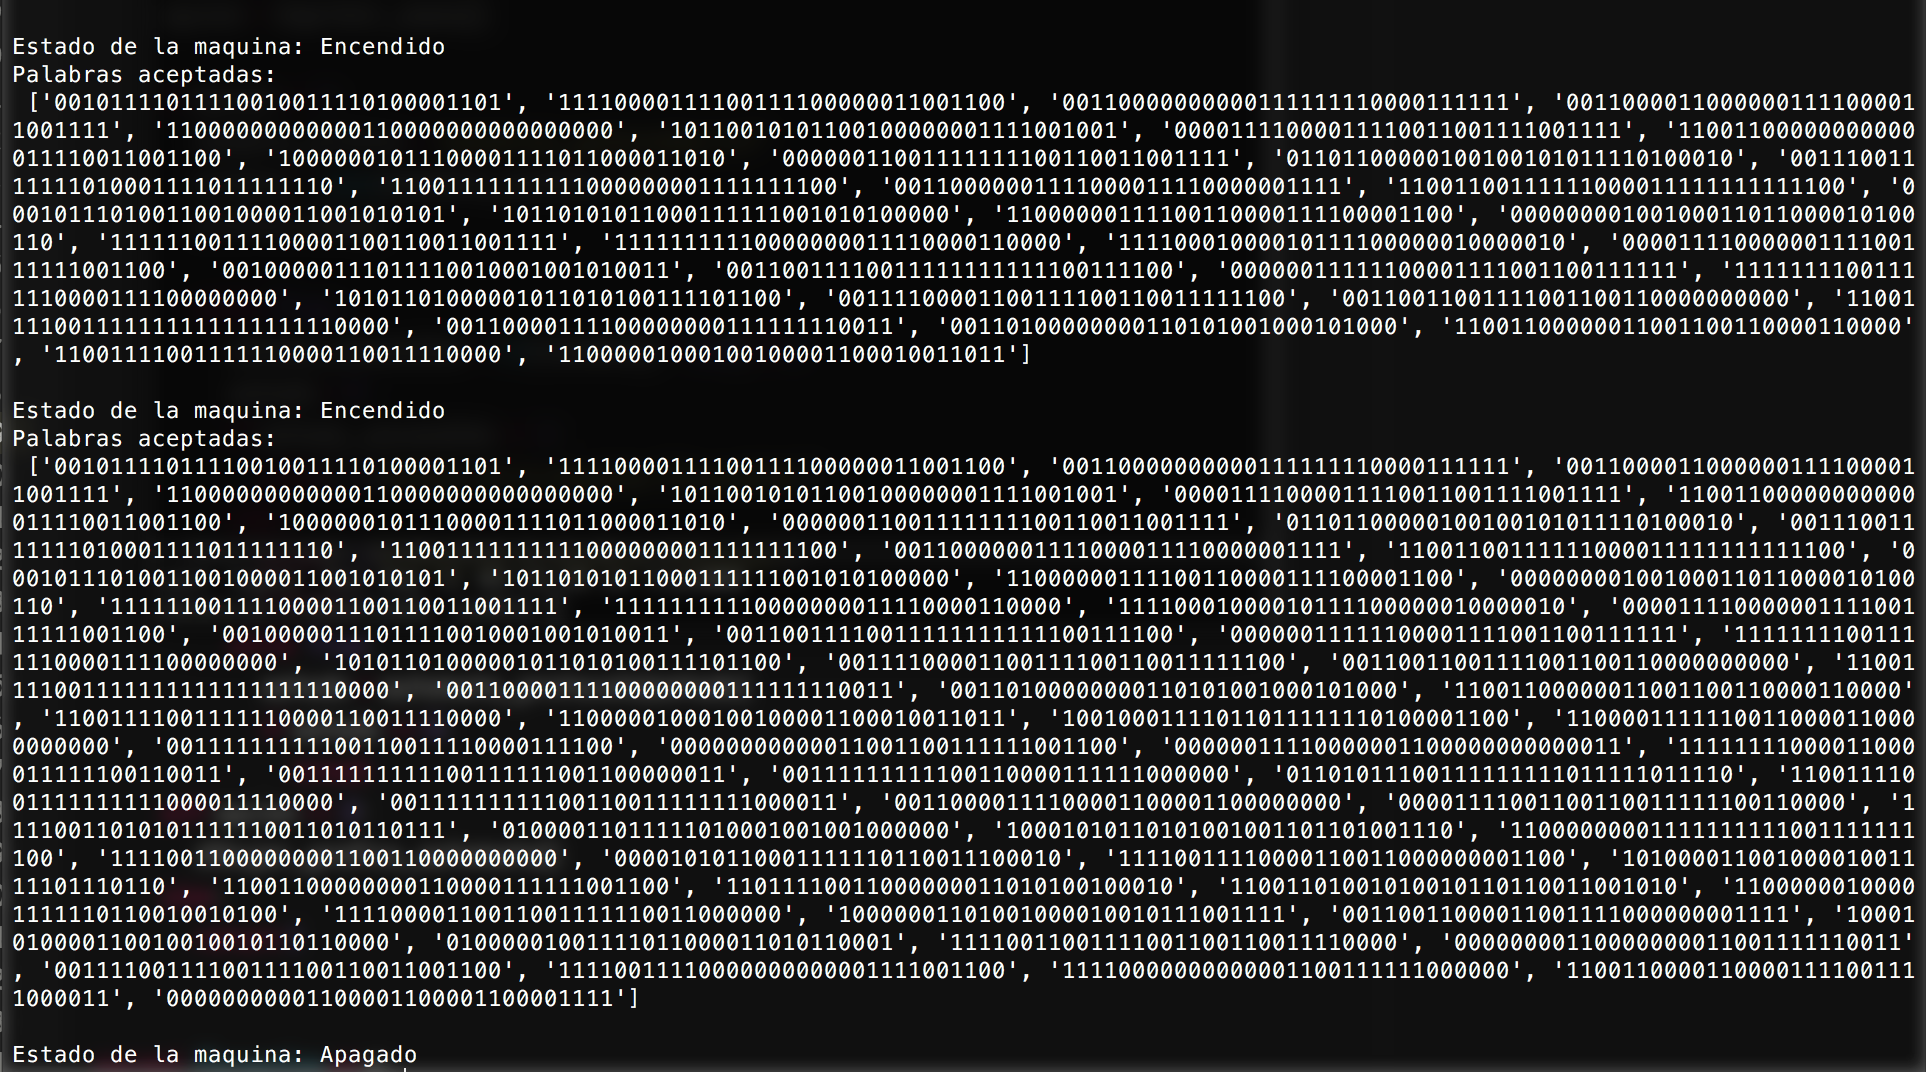
\includegraphics[width=\textwidth, height=7cm]{protocolo_encender}
\caption{El programa corriendo el protocolo.}
\label{fig:automata_protocolo_encender}
\end{figure}

\begin{figure}[H]
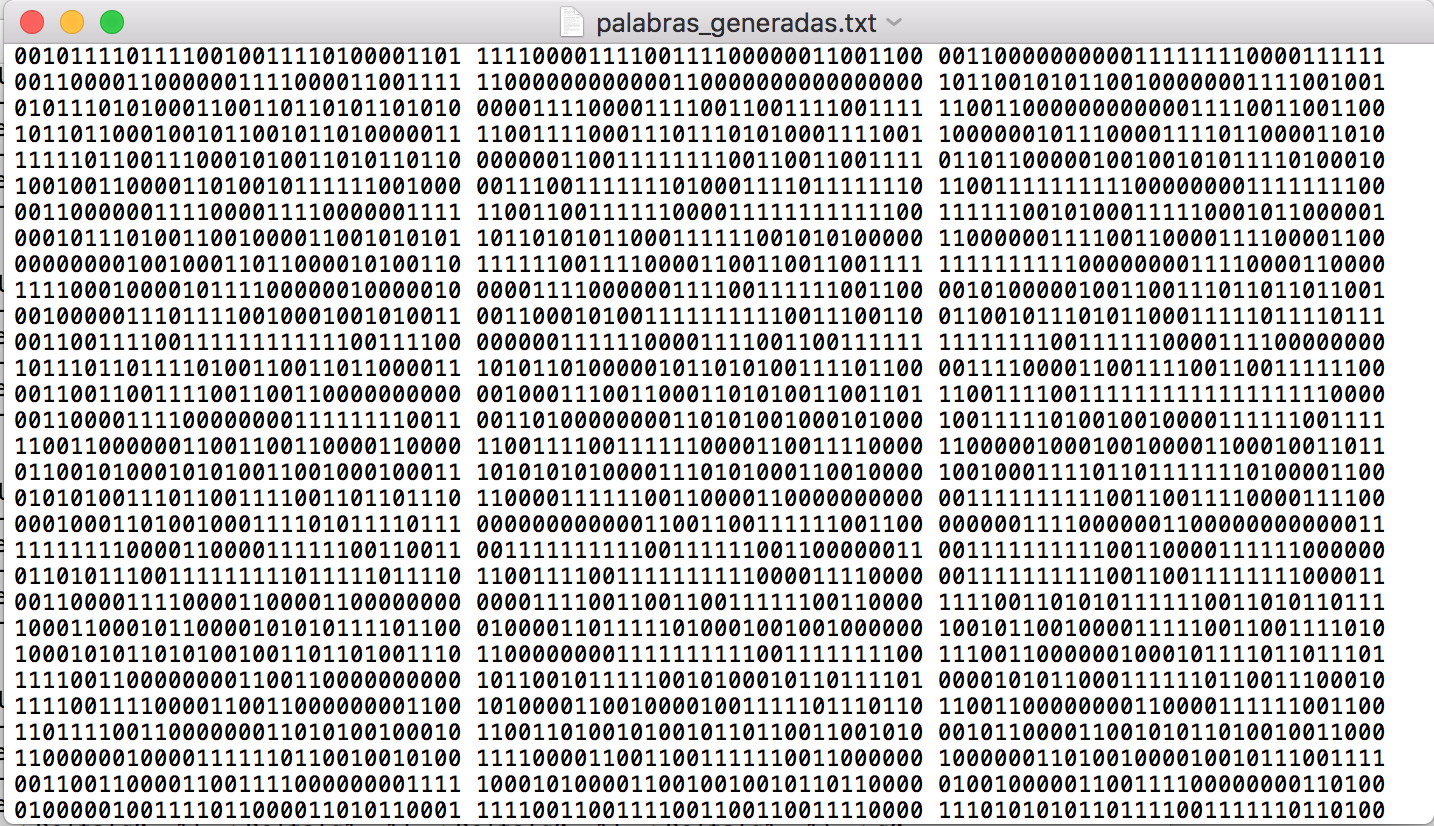
\includegraphics[width=\textwidth, height=7cm]{protocolo_generadas}
\caption{Las palabras generadas por el programa.}
\label{fig:automata_protocolo_generadas}
\end{figure}

\begin{figure}[H]
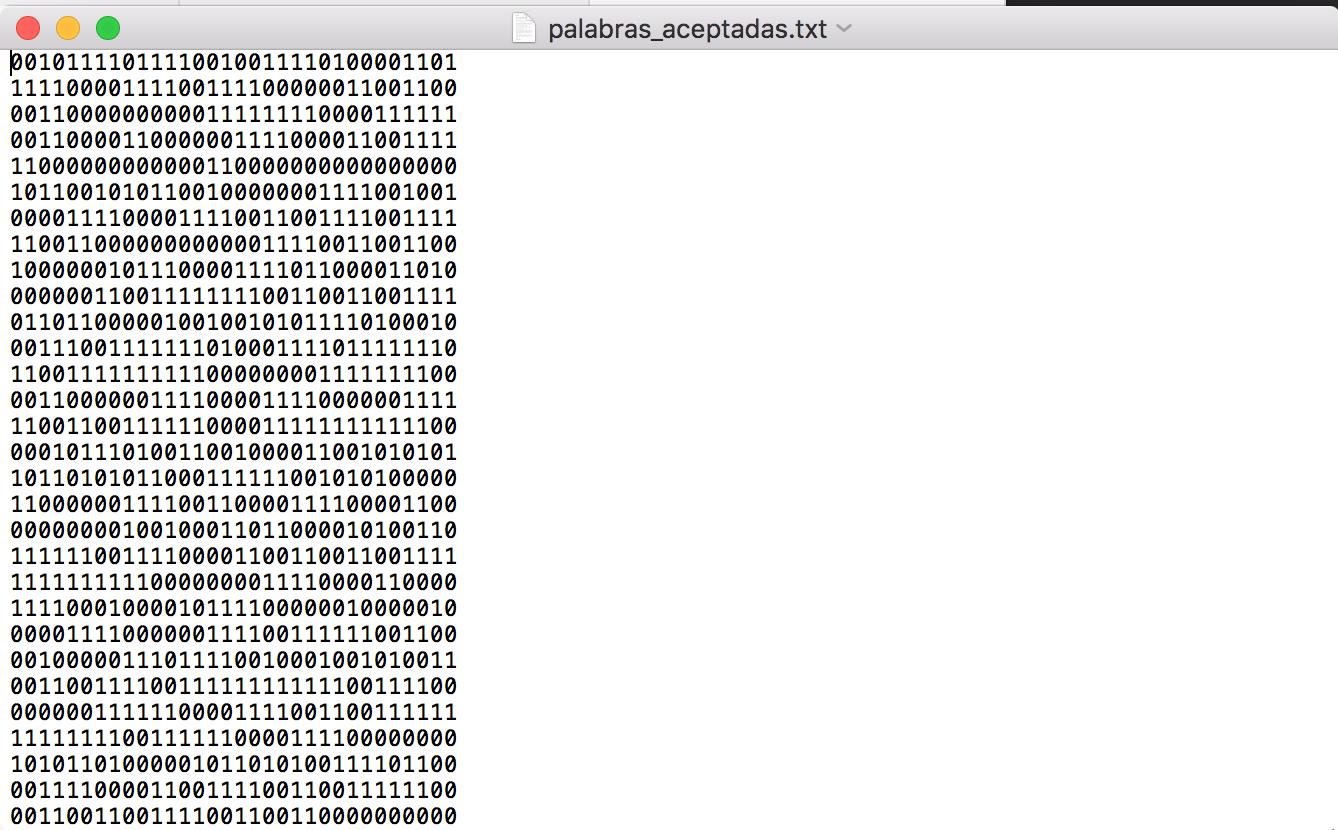
\includegraphics[width=\textwidth, height=7cm]{protocolo_aceptadas}
\caption{Las palabras aceptadas según el criterio de paridad.}
\label{fig:automata_protocolo_aceptadas}
\end{figure}

\begin{figure}[H]
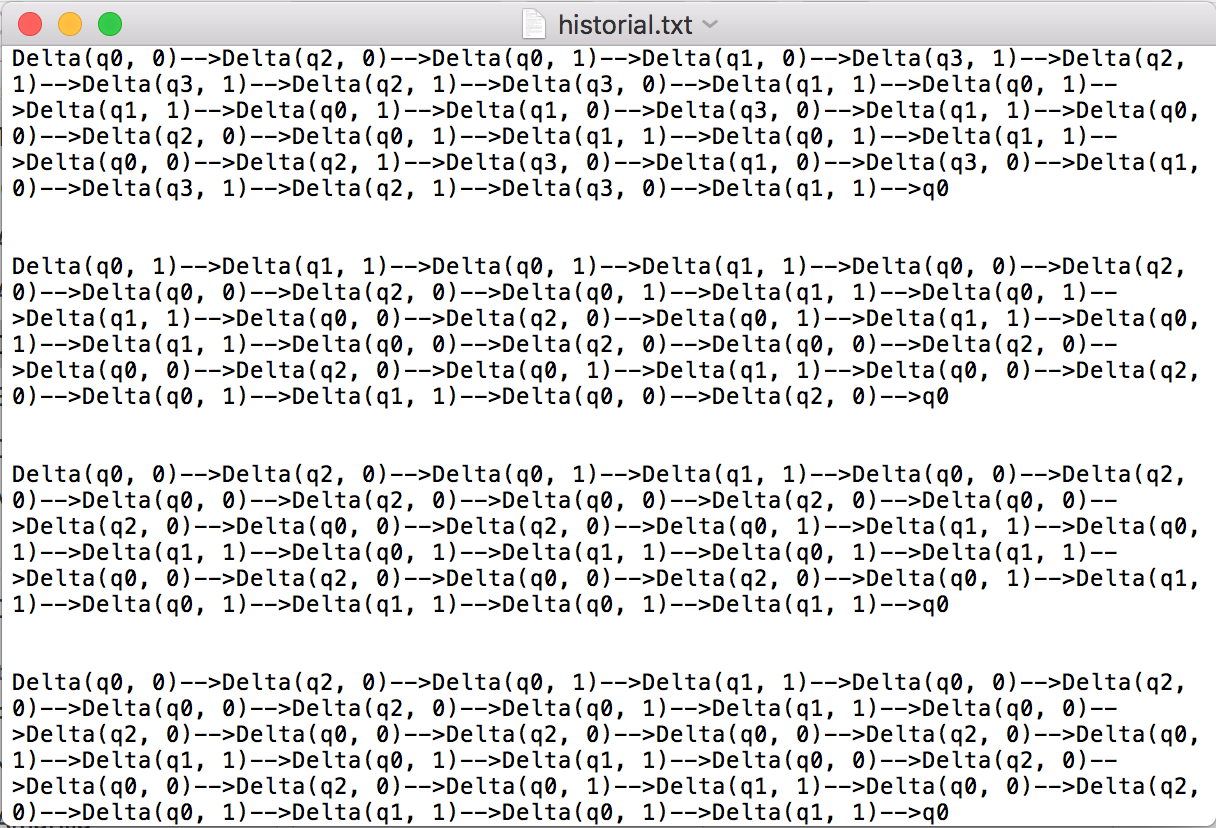
\includegraphics[width=\textwidth, height=7cm]{protocolo_historial}
\caption{El historial de estados del autómata de paridad usado para validar las palabras.}
\label{fig:automata_protocolo_historial}
\end{figure}

\begin{figure}[H]
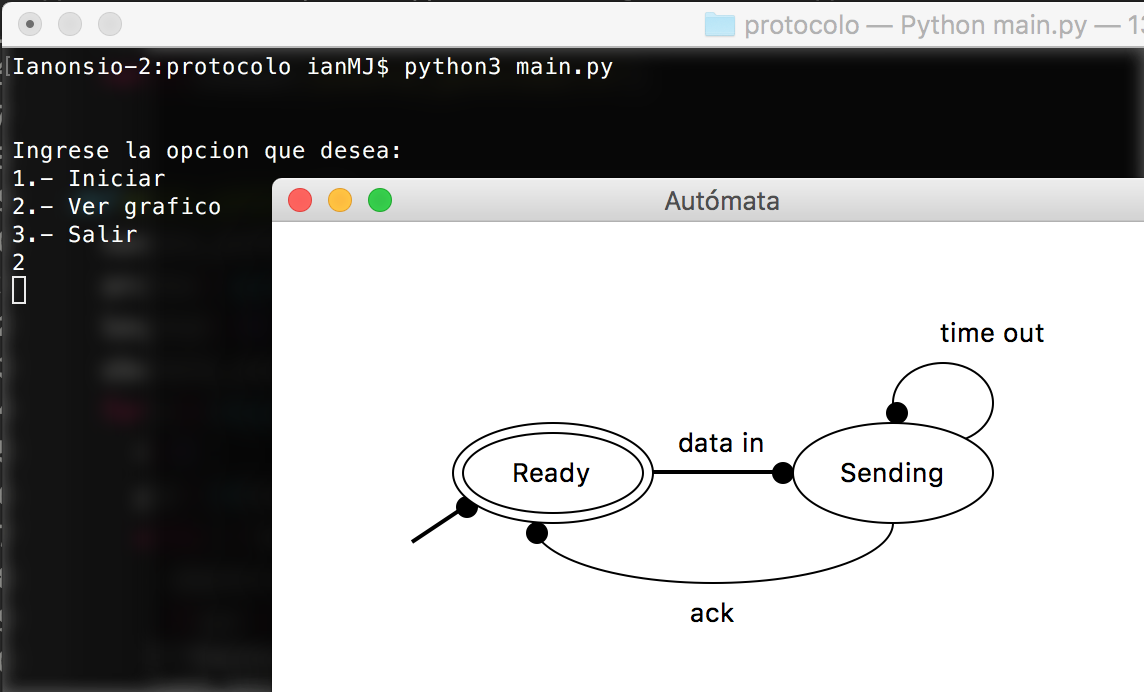
\includegraphics[width=\textwidth, height=7cm]{automata_protocolo_prueba}
\caption{El programa imprimiendo el autómata.}
\label{fig:automata_protocolo_prueba}
\end{figure}

%===============================================================================================
%===============================================================================================
%===============================================================================================
%===============================================================================================
%===============================================================================================
%===============================================================================================
%===============================================================================================

\newpage
\section{Cadenas que terminan en 01}
Los autómatas no determínisticos (NFA) son otro tipo de autómatas cuya característica es que cada estado puede ser seguido de un conjunto de estados, a diferencia de los autómatas determinísticos que son lineales. Otra característica importante es que los NFA es que tienen menos caminos que los DFA, el siguiente problema, ilustra la utilidad de este tipo de autómatas.

\subsection{Descripción del problema}
Se necesita crear un programa que sea capaz de evaluar si una cadena binaria termina en \textit{01}. Además, tiene que imprimir una tabla con los estados por los que ha pasado la cadena a evaluar.

\subsection{Código}
El autómata utilizado para este problema fue:

\begin{figure}[H]
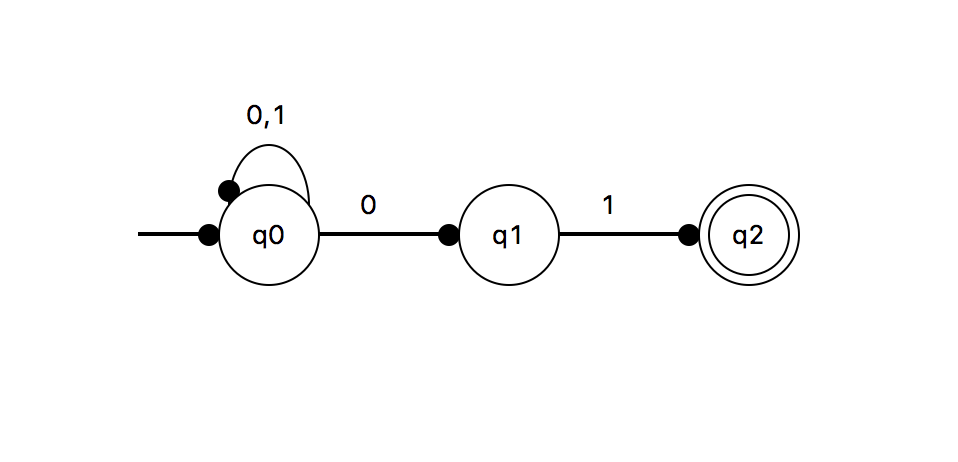
\includegraphics[width=\textwidth, height=10cm]{automata_cero_uno}
\caption{El autómata utilizado para este problema.}
\label{fig:automata_cero_uno_modelo}
\end{figure}

El lenguaje utilizado para este programa fue Python en su versión 3.5. El código para resolver el problema es el siguiente:\\

Archivo: main\_cero\_uno.py
\lstset{language=Python, breaklines=true, basicstyle=\footnotesize}
\begin{lstlisting}[frame=single]
from metodos import *

def main():
    try:
    	   historial = open('historial_cero_uno.txt','w')
    	   historial.close()
        
        while True:
            opcion = imprimir_menu()
            texto = ''
            tabla_estados = []
            if opcion == 1:
                while True:
                    texto = input('\n\nIngrese una palabra binaria para evaluar: ')
                    tabla_estados = evaluar_cadena(texto)
                    imprimir_estados(tabla_estados)

                    opcion = input("\n\nQuiere ingresar otro numero? [s/n]  ")
                    if opcion != 's' and opcion != 'S':
                        break

            elif opcion == 2:
                aleatorio = 0
                while True:
                    texto = generar_palabra()
                    print('\n\nSe evaluara la palabra: ', texto)
                    tabla_estados = evaluar_cadena(texto)
                    imprimir_estados(tabla_estados)
                    aleatorio = int(random() * 10) % 2
                    if aleatorio == 0:
                        break
            elif opcion == 3:
                graficar_automata()
            else:
                return 1

    except Exception as e:
        print('Uuups, parece que hubo un problema, ', e)


def imprimir_menu():
    seguir = True
    while seguir:
        try:
            opcion = int(input("\n\nIngrese la opcion que desea: \n1.- Ingresar texto \n2.- Automatico \n3.- Ver grafico del automata \n4.- Salir\n"))
            return opcion
        except Exception as e:
            print("Por favor, ingrese un dato valido.")


main()

\end{lstlisting}

\vspace{1em}

Archivo: metodos\_cero\_uno.py
\lstset{language=Python, breaklines=true, basicstyle=\footnotesize}
\begin{lstlisting}[frame=single]
from random import random
from tkinter import *

def evaluar_cadena(texto):
    tabla_estados = [[0]]
    estado = []
    contador = 0
    for x in texto:
        for i in range(len(tabla_estados)):
            estado = automata(tabla_estados[i][contador], x)
            if len(estado) == 2:
                tabla_estados.append([0] * (contador+1))
                tabla_estados[(len(tabla_estados)-1)].append(1)
                tabla_estados[i].append(0)
            elif estado[0] == 2:
                tabla_estados[i].append(2)
            elif estado[0] == -1:
                tabla_estados[i].append(-1)
            else:
                tabla_estados[i].append(0)

        contador += 1

    return tabla_estados


def automata(estado, letra):
    if estado == 0:
        return estado_cero(letra)
    elif estado  == 1:
        return estado_uno(letra)
    elif estado == 2:
        return estado_dos(letra)
    else:
        return [-1]


def estado_cero(letra):
    if letra == '0':
        return [0,1]
    elif letra == '1':
        return [1]
    else:
        return [-1]



def estado_uno(letra):
    if letra == '1':
        return [2]
    else:
        return [-1]



def estado_dos(letra):
    if letra != '':
        return [-1]
    else:
        return [2]



def imprimir_estados(tabla_estados):
    archivo = open('historial_cero_uno.txt', 'a')
    auxiliar = ''
    for x in range(0,len(tabla_estados[0])):
        for j in range(len(tabla_estados)):
            if tabla_estados[j][x] == -1:
                archivo.write('xx ')
                print('xx', end=' ')
            else:
                auxiliar = 'q'+str(tabla_estados[j][x])+' '
                archivo.write(auxiliar)
                print(auxiliar, end='')

        archivo.write('\n')
        print("")

    if tabla_estados[len(tabla_estados)-1][len(tabla_estados[0])-1] == 2:
        archivo.write('La palabra es valida\n\n')
        print("La palabra es valida\n\n")
    else:
        archivo.write('La palabra no es valida\n\n')
        print("La palabra no es valida\n\n")

    archivo.close()


def graficar_automata():
    raiz = Tk()
    raiz.title('Automata')
    raiz.geometry('500x250')
    canvas = Canvas(raiz, width=600, height=410, bg='white')
    canvas.place(x=0,y=0)
    canvas.pack(expand=YES, fill=BOTH)

    x = 120
    y = 100
    r = 50
    numero_circulos = 3
    opciones = ['0','1']
    canvas.create_line(x-40, y+(r/2), x, y+(r/2), width=2, fill='black')
    canvas.create_oval(x-10, y+(r/2)-5, x, y+(r/2)+5, width=1, fill='black')

    xy = x+5, y-20, x+45, y+40
    canvas.create_arc(xy, start=0, extent=180, style='arc')
    canvas.create_oval(x, y+(r/2)-27, x+10, y+(r/2)-17, width=1, fill='black')
    widget = Label(canvas, text='0,1', fg='black', bg='white')
    widget.pack()
    canvas.create_window(x+25, y-35, window=widget)

    for i in range(numero_circulos):
        canvas.create_oval(x, y, x+r, y+r, width=1, fill='white')
        widget = Label(canvas, text='q'+str(i), fg='black', bg='white')
        widget.pack()
        canvas.create_window(x+.5*r, y+.5*r, window=widget)

        if i < numero_circulos-1:
            canvas.create_line(x+r, y+(r/2), x+r+70, y+(r/2), width=2, fill='black')
            widget = Label(canvas, text=opciones[i], fg='black', bg='white')
            widget.pack()
            canvas.create_window(x+r+25, y+(r/2)-15, window=widget)
            canvas.create_oval(x+r+60, y+(r/2)-5, x+r+70, y+(r/2)+5, width=1, fill='black')

        if i == numero_circulos -1:
            canvas.create_oval(x+5, y+5, x+r-5, y+r-5, width=1, fill='white')
        x += r+70

    raiz.mainloop()

\end{lstlisting}

\newpage
\subsection{Pruebas}
En este apartado se muestran las imágenes de los resultados del autómata.

\begin{figure}[H]
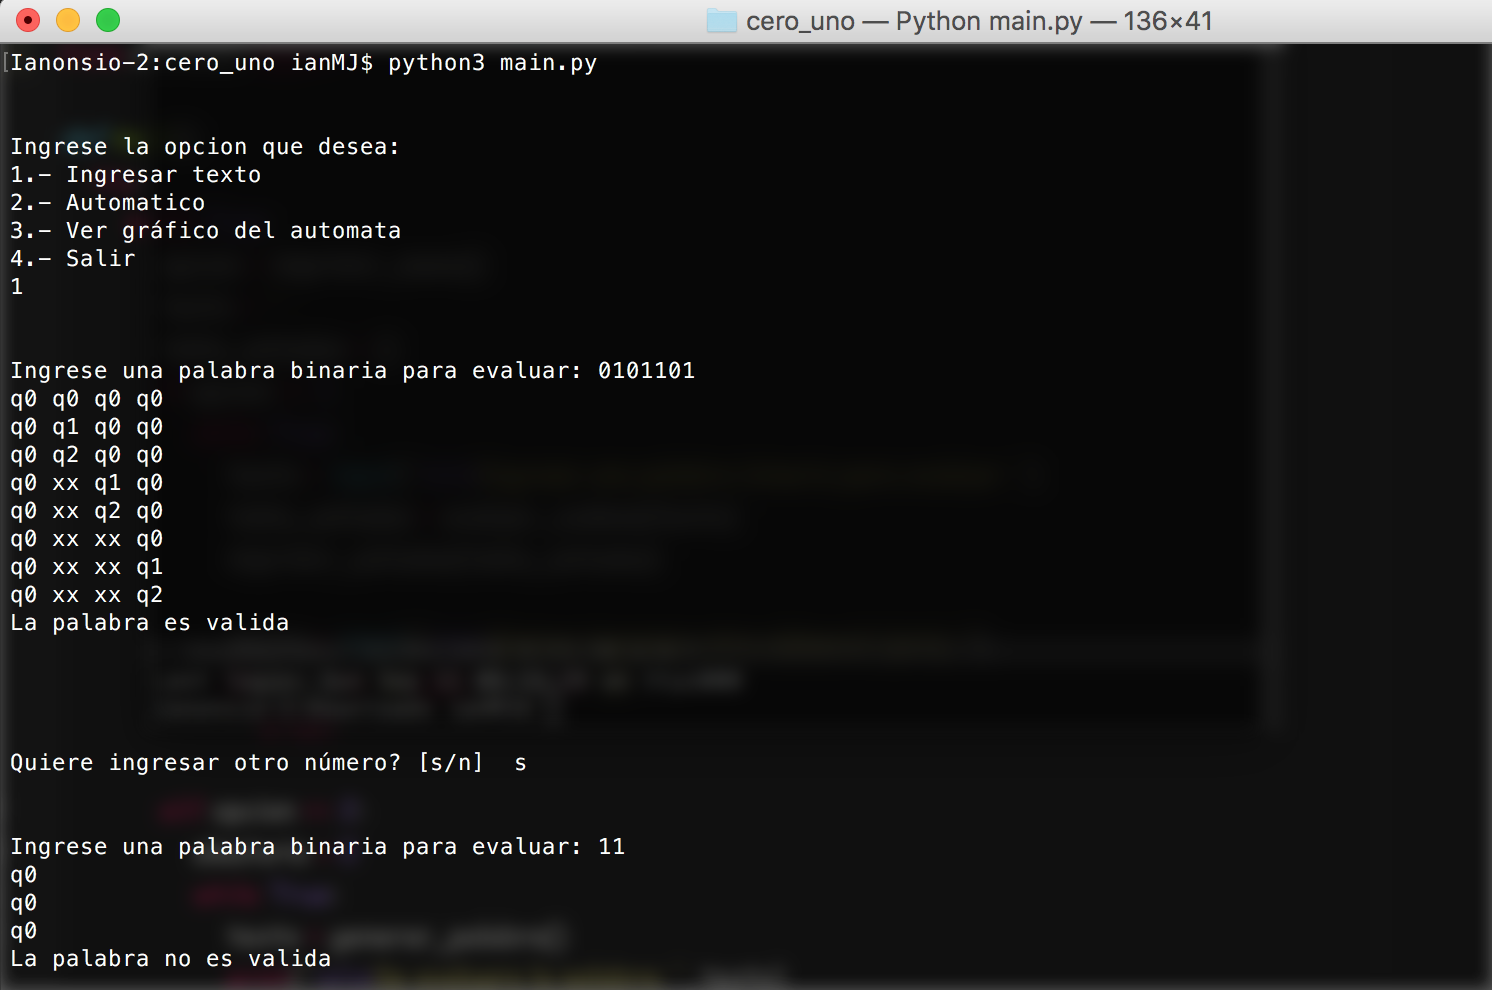
\includegraphics[width=\textwidth, height=8cm]{cero_uno_manual}
\caption{Números ingresados manualmente.}
\label{fig:automata_cero_uno_texto}
\end{figure}

\begin{figure}[H]
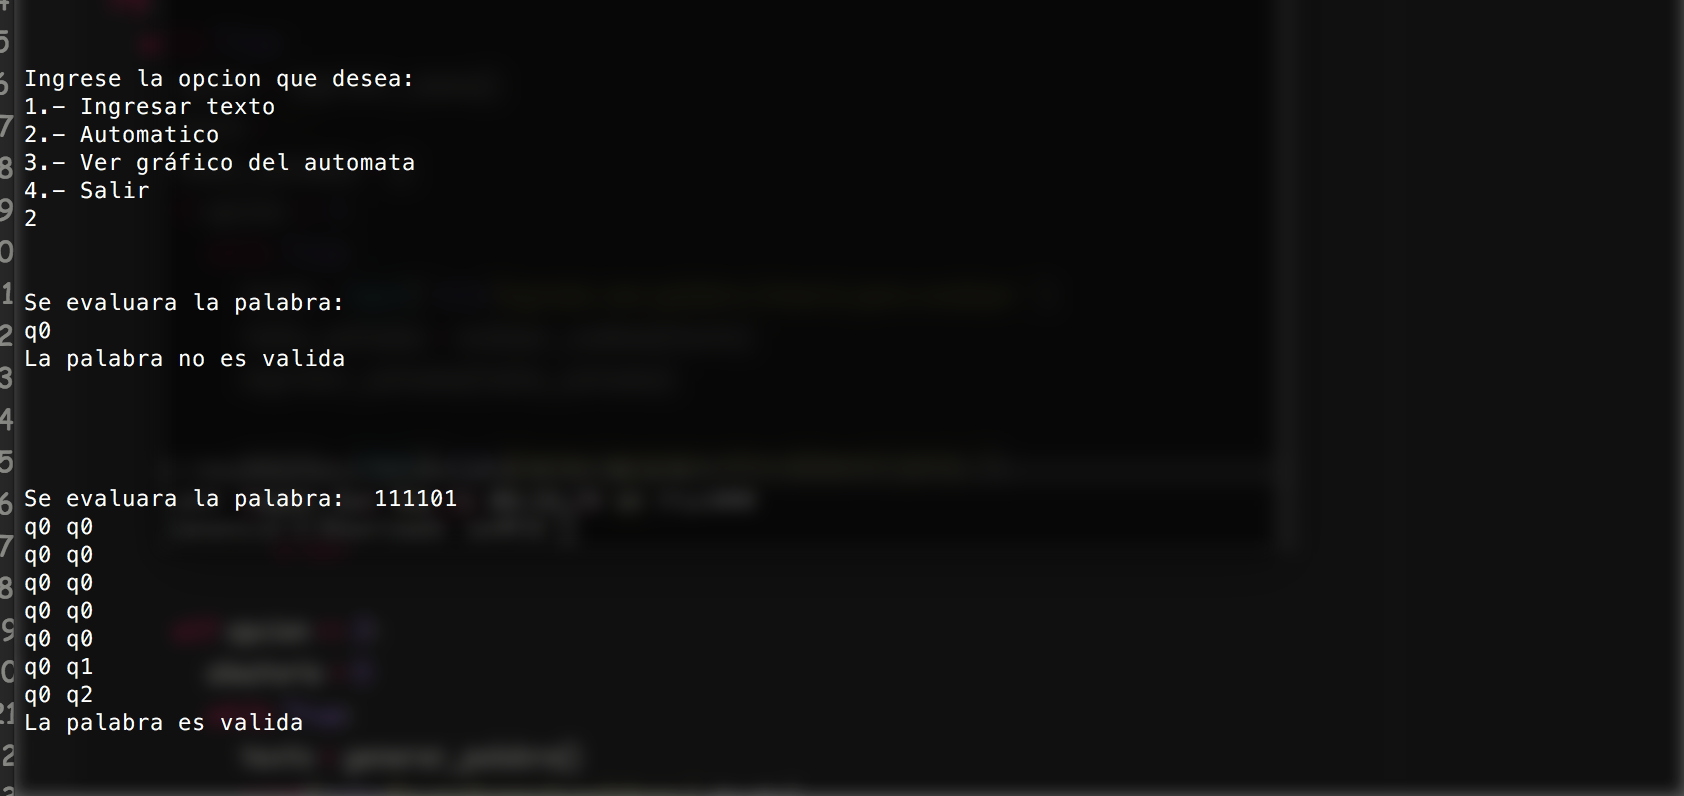
\includegraphics[width=\textwidth, height=8cm]{cero_uno_auto}
\caption{Modo automático.}
\label{fig:automata_cero_uno_auto}
\end{figure}

\begin{figure}[H]
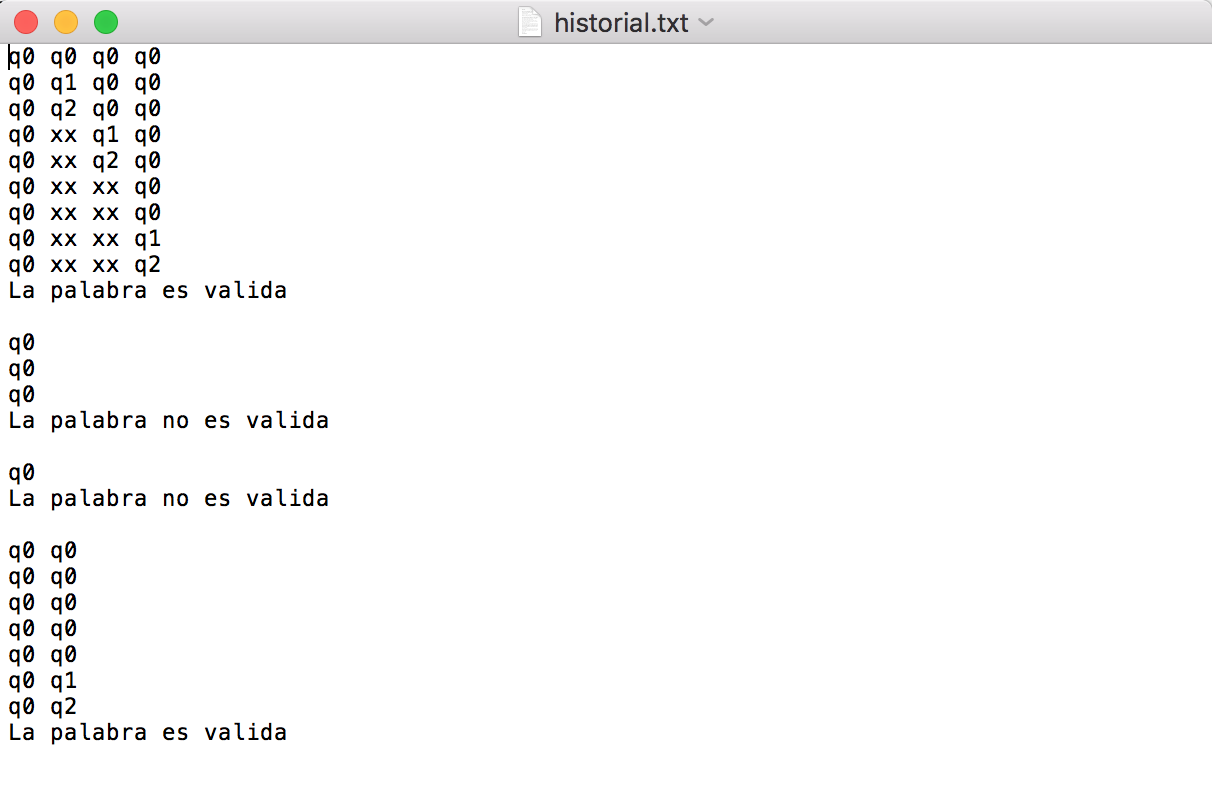
\includegraphics[width=\textwidth, height=8cm]{cero_uno_historial}
\caption{El historial de correr el programa.}
\label{fig:automata_cero_uno_historial}
\end{figure}

\begin{figure}[H]
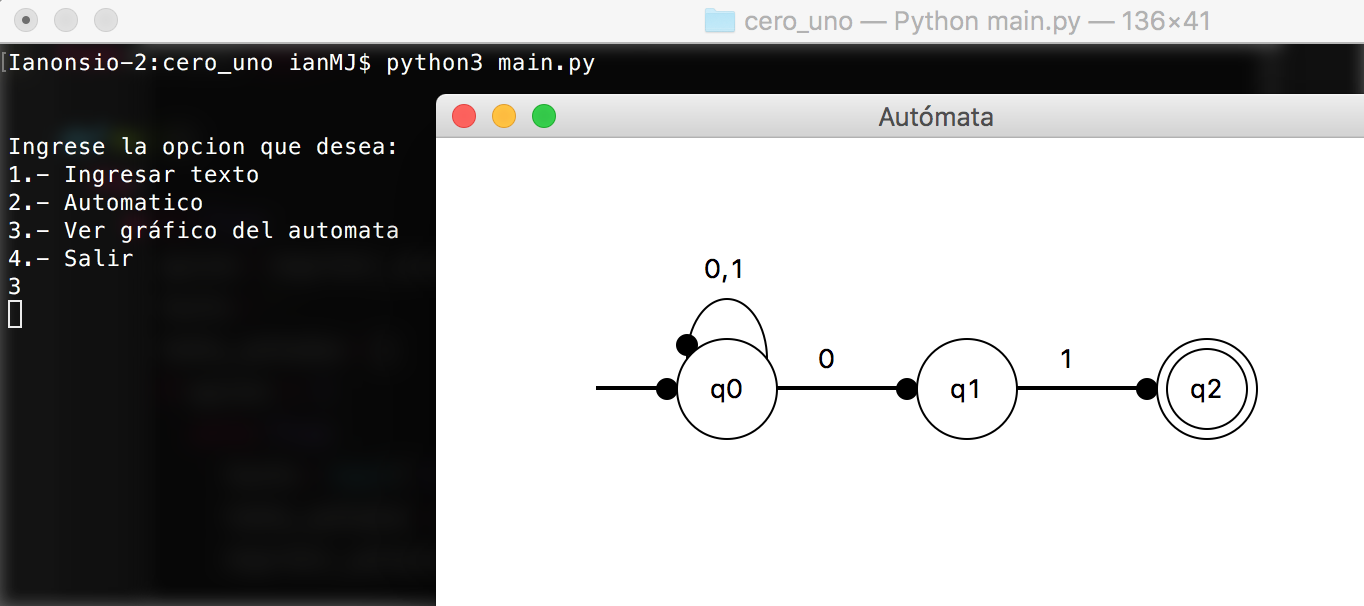
\includegraphics[width=\textwidth, height=8cm]{automata_cero_uno_prueba}
\caption{El programa imprimiendo el autómata.}
\label{fig:automata_cero_uno_prueba}
\end{figure}


%===============================================================================================
%===============================================================================================
%===============================================================================================
%===============================================================================================
%===============================================================================================
%===============================================================================================
%===============================================================================================
\newpage

\bibliographystyle{acm}
\bibliography{bibliografia}

\end{document}
